\documentclass[aspectratio=169]{beamer}
\usepackage{color,amsmath}
\usepackage{subfigure}
\usepackage{booktabs}
\usepackage{framed}
\usepackage{comment}

\def\vf{\vfill}

%%%%%%%%%%%%%%%%%%%%%%%%%%
\title[]{Linking survey data to other data\\(03-05)}
\author[]{Matthew J. Salganik\\Department of Sociology\\Princeton University}
\date[]{Soc 596: Computational Social Science\\Fall 2016
\vfill
\begin{flushright}
\vspace{0.6in}

\includegraphics[width=0.1\textwidth]{figures/cc.png}
\end{flushright}
}
\begin{document}
%%%%%%%%%%%%%%%%%%%%%%%%%%
\frame{\titlepage}
%%%%%%%%%%%%%%%%%%%%%%%%%%
\begin{frame}

\begin{center}
\small{
\begin{tabular}{ l c c c}
           & Sampling & Interviews & Data environment\\
\hline
1st era & Area probability & Face-to-face & Stand-alone \\
2nd era & \parbox[t]{3cm}{\centering Random digital dial\\probability} & Telephone & Stand-alone \\
3rd era & Non-probability & Computer-administered & \textcolor{blue}{Linked} \\
\end{tabular}
}
\end{center}

\end{frame}
%%%%%%%%%%%%%%%%%%%%%%%%%%%
\begin{frame}

\begin{center}
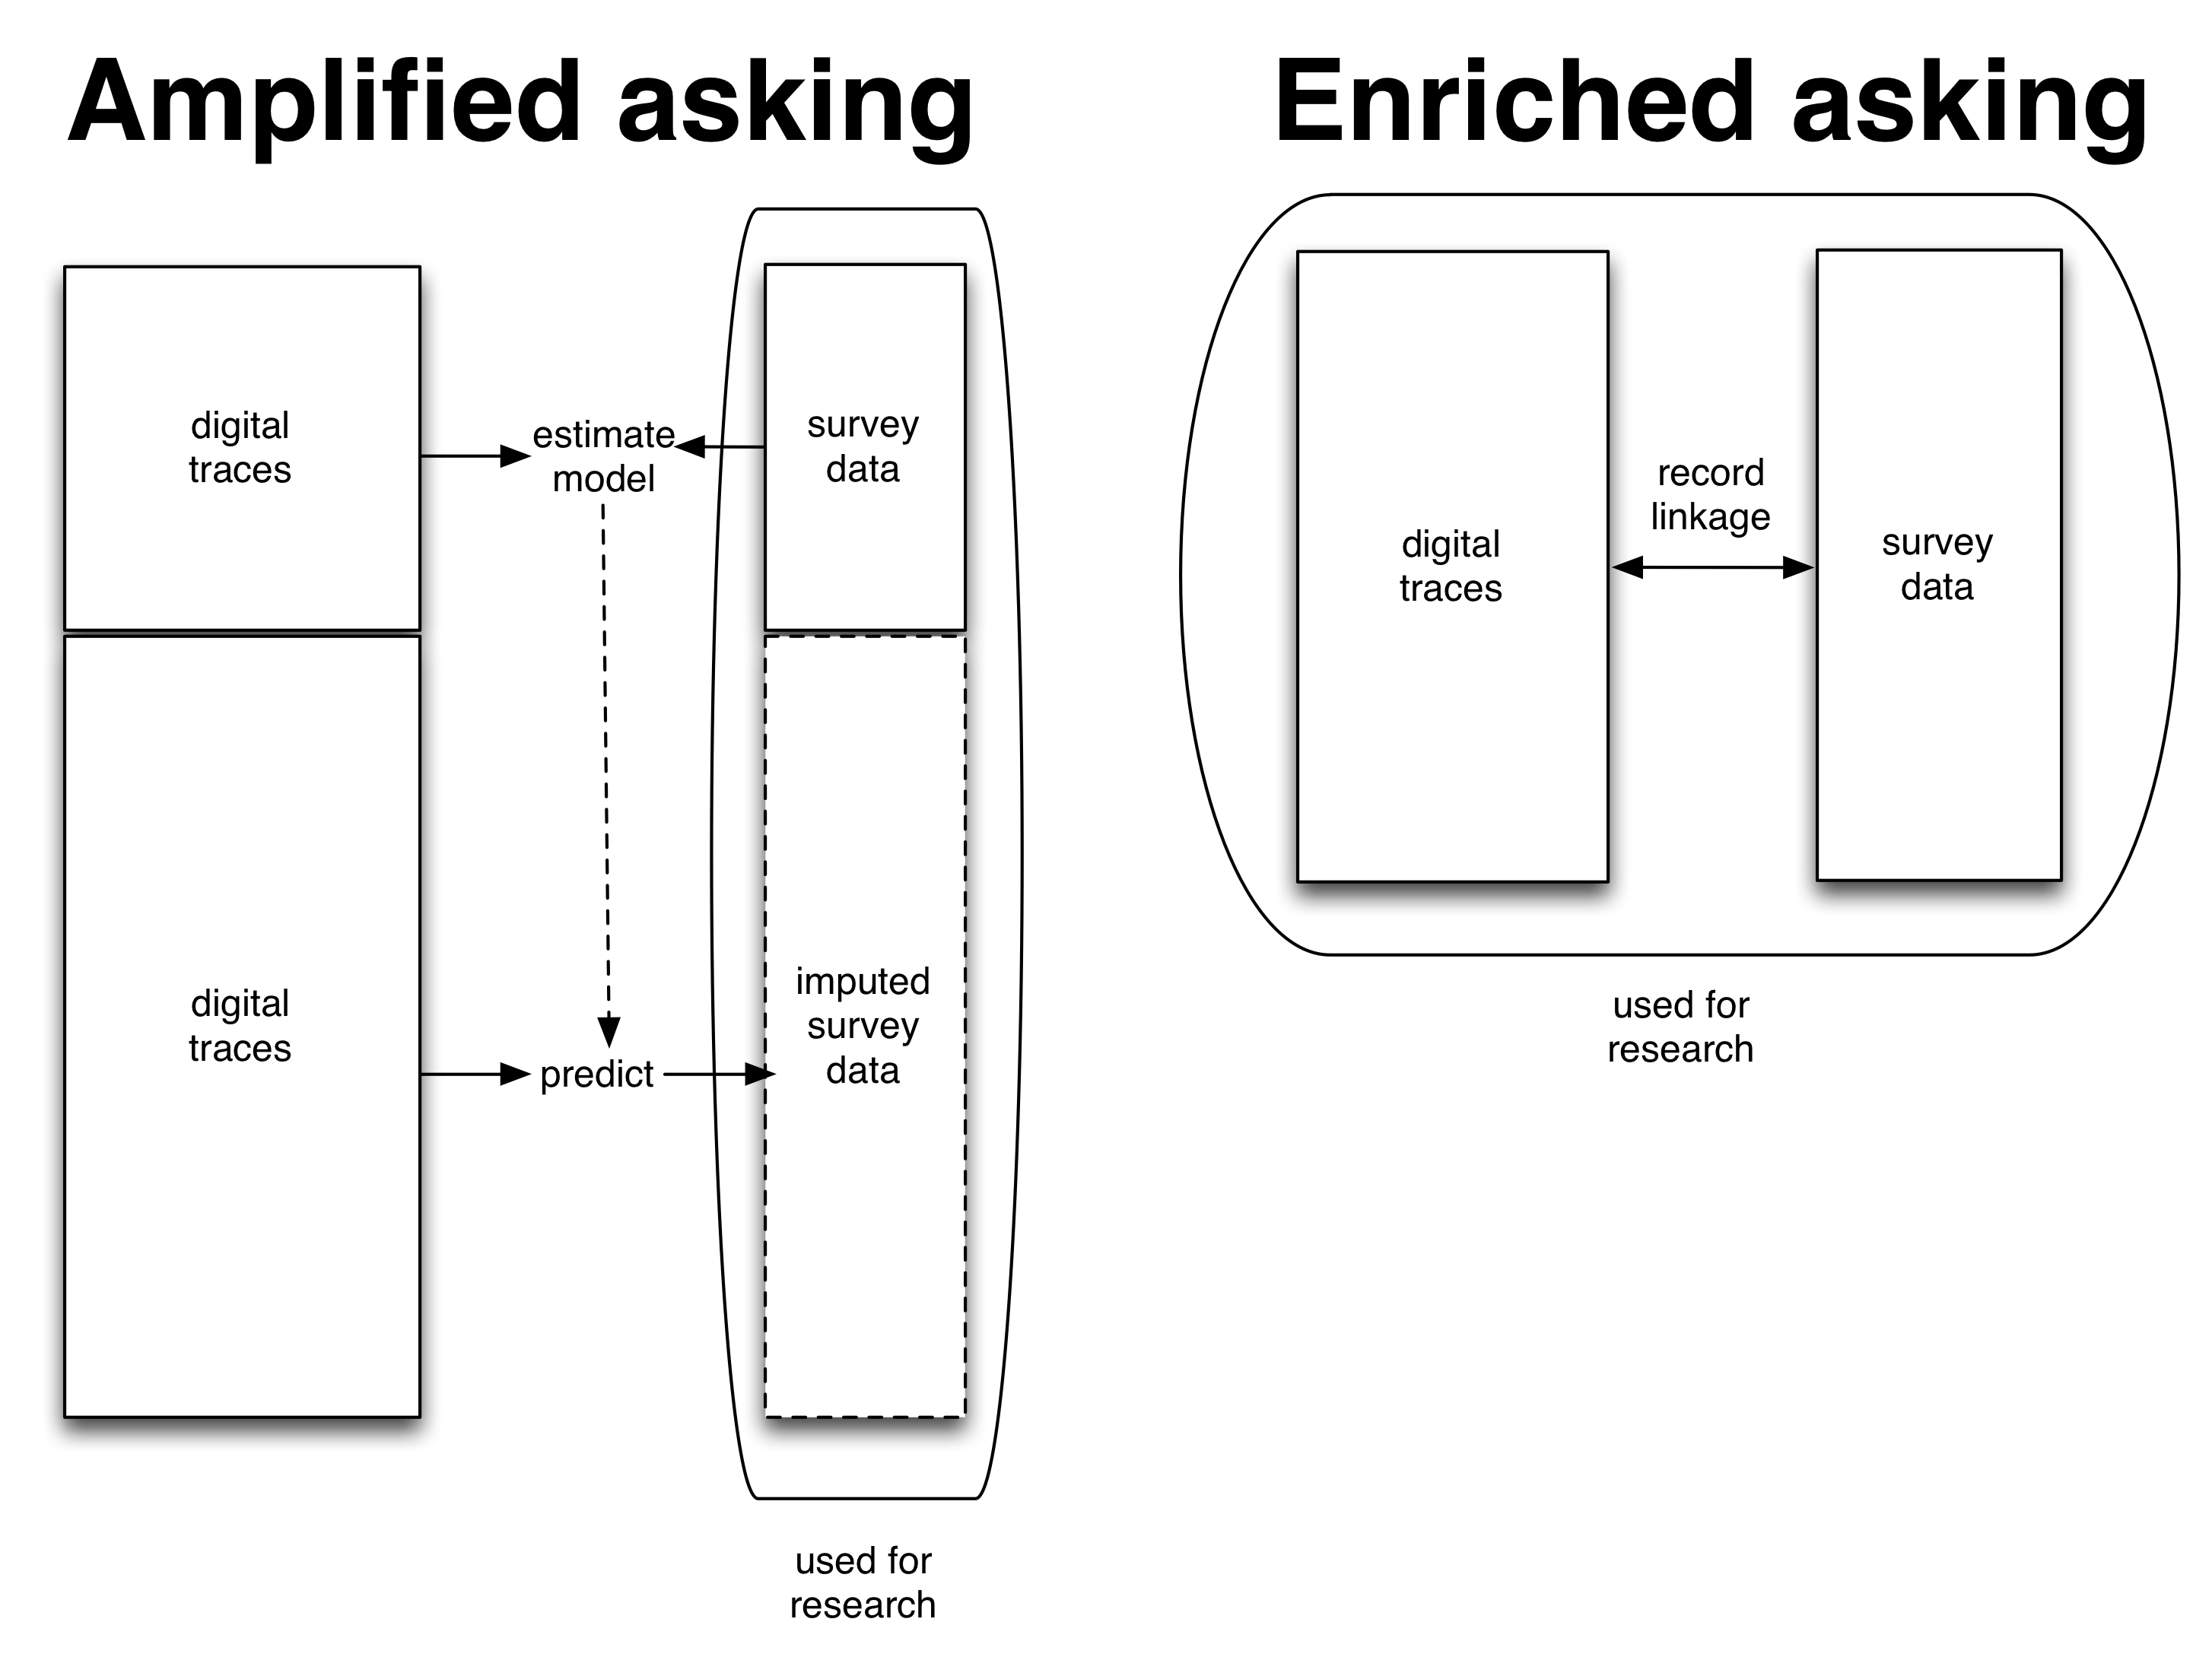
\includegraphics[width=0.6\textwidth]{figures/found_survey_combined}
\end{center}

Note the different role of the big data in each case

\end{frame}
%%%%%%%%%%%%%%%%%%%%%%%%%%%
\begin{frame}

\begin{center}
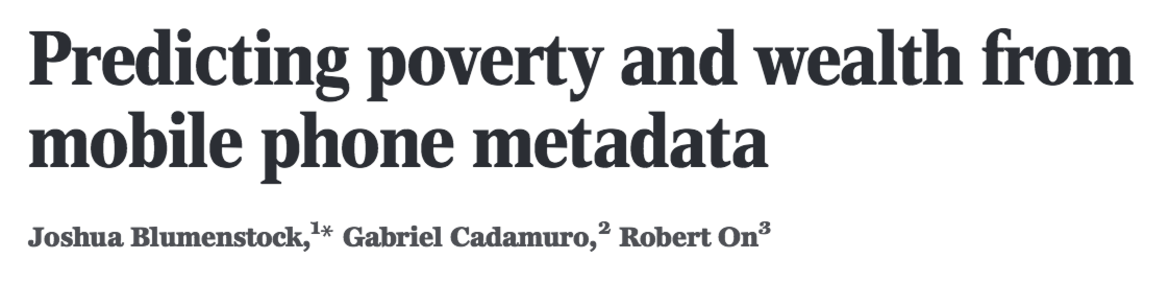
\includegraphics[width=0.9\textwidth]{figures/blumenstock_predicting_2015_title}
\end{center}

\end{frame}
%%%%%%%%%%%%%%%%%%%%%%%%%%%
\begin{frame}

\begin{center}
\only<1>{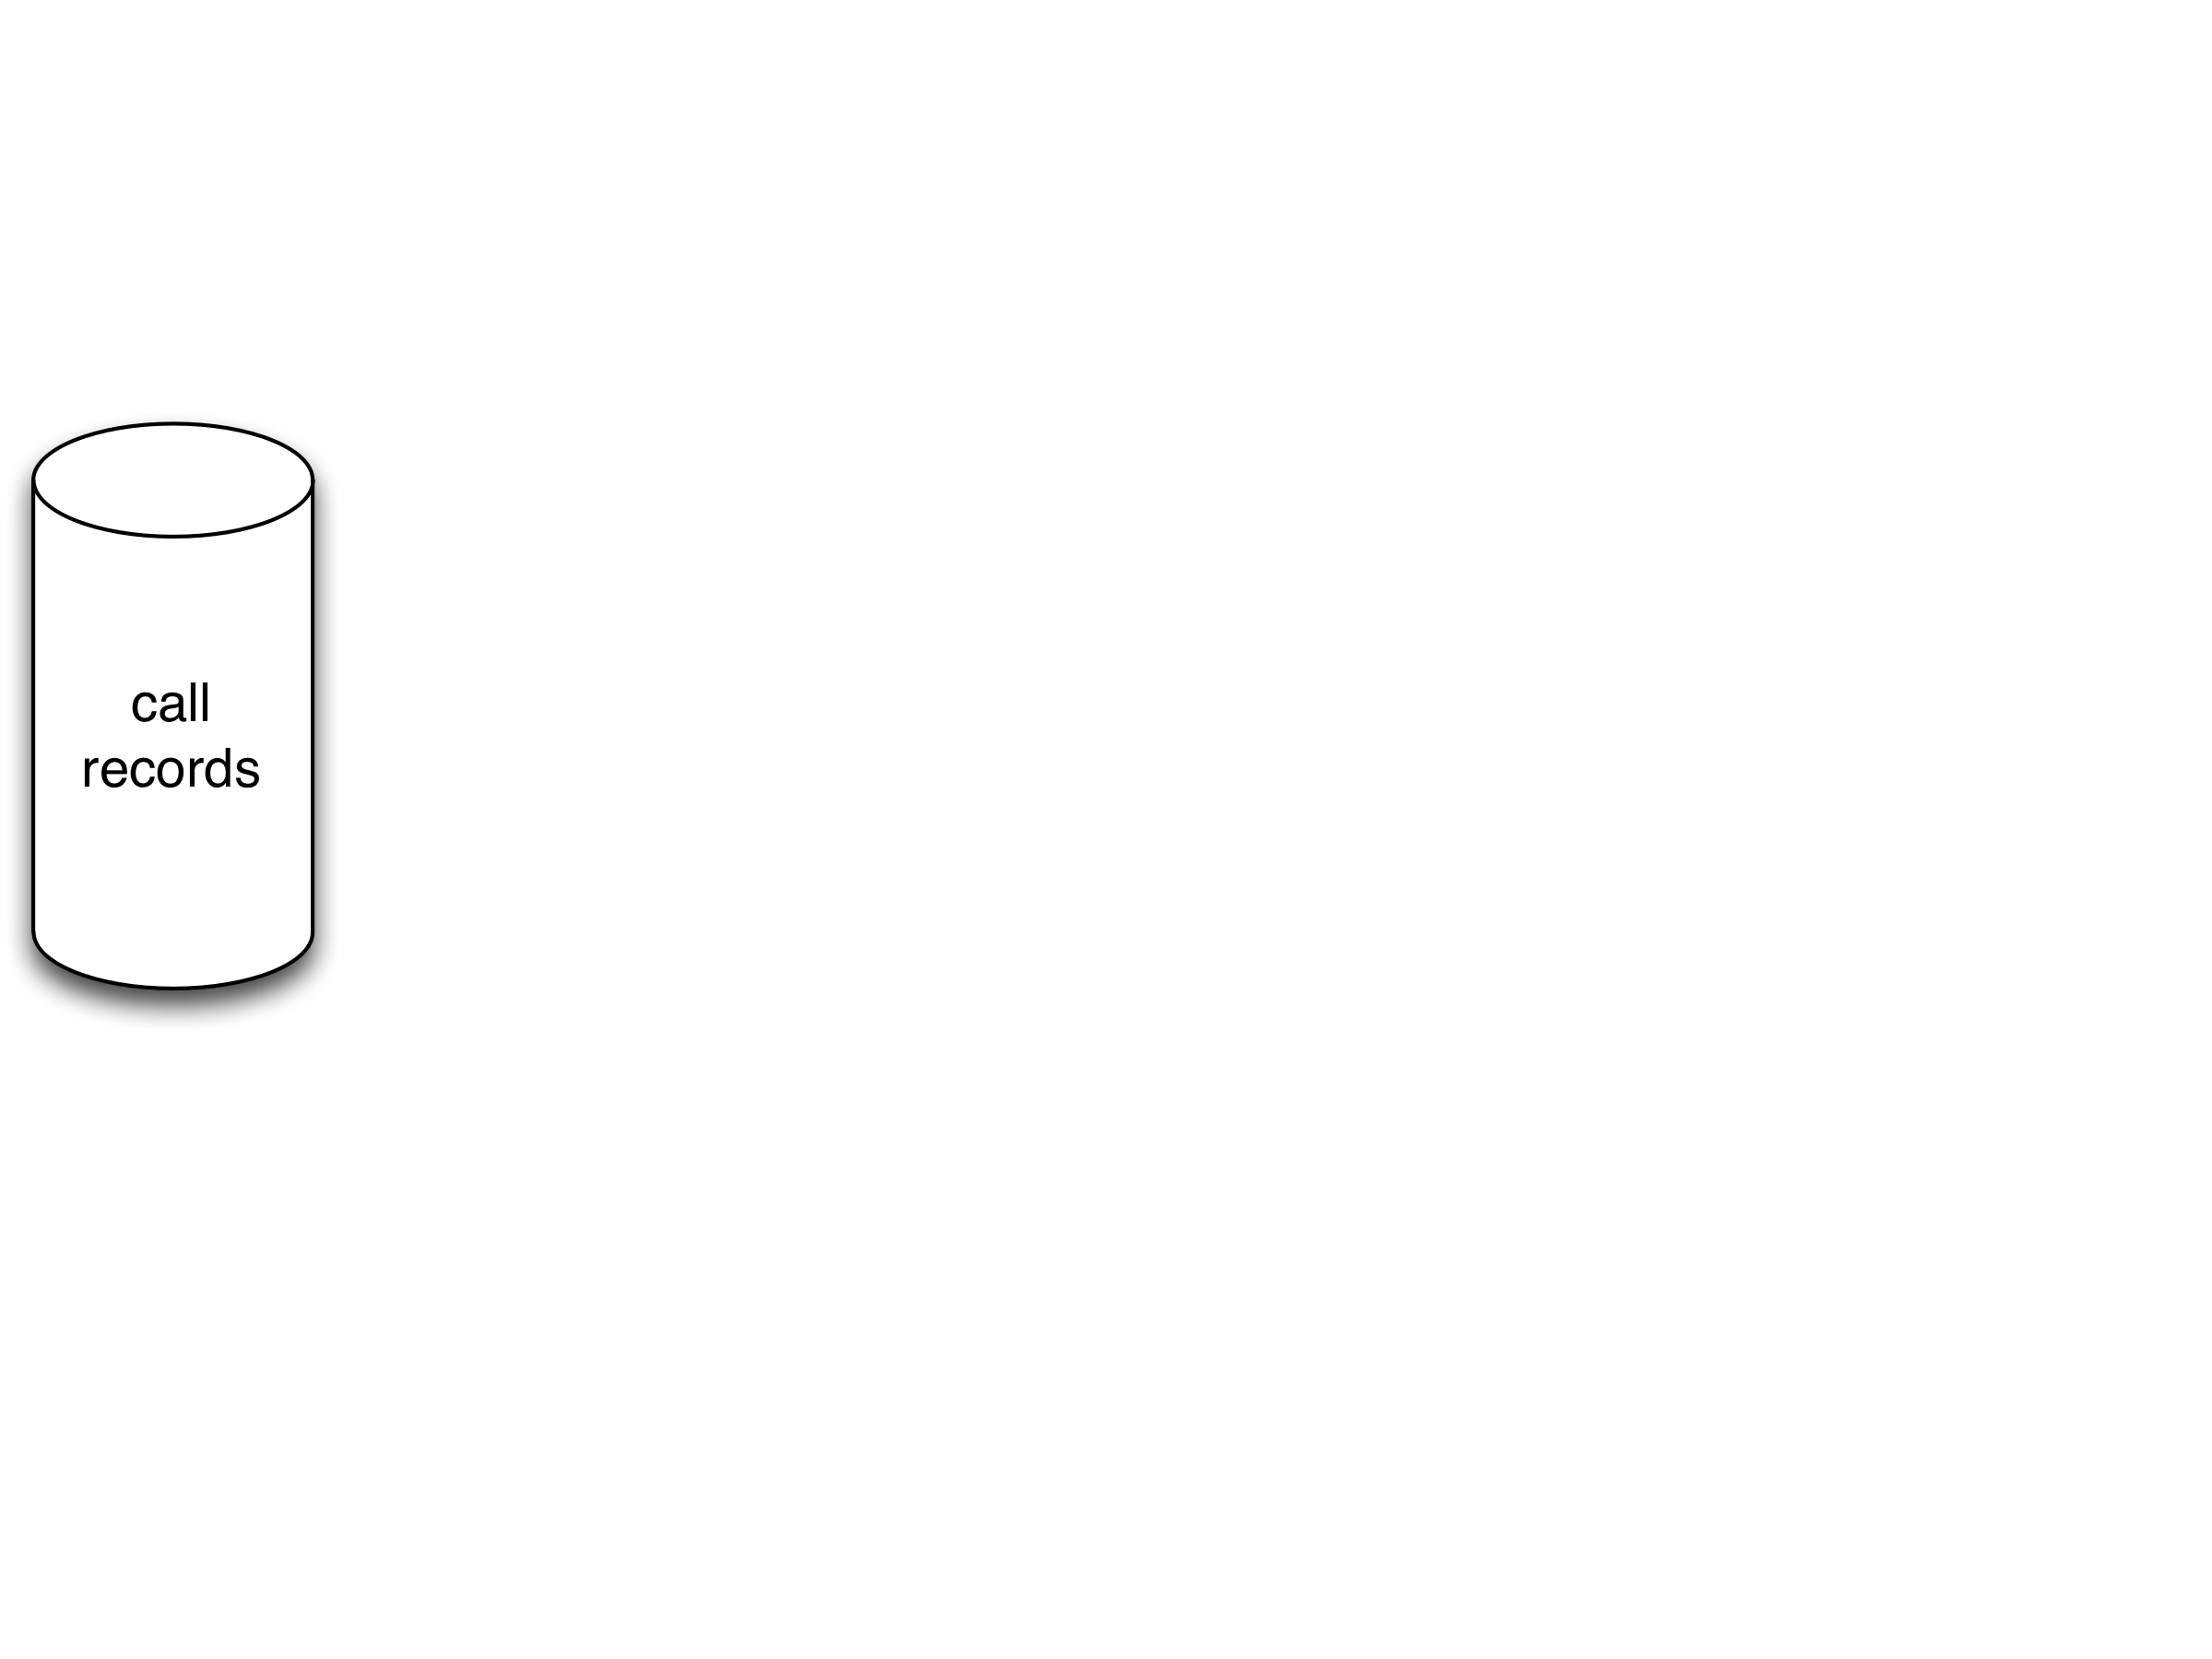
\includegraphics[width=0.7\textwidth]{figures/blumenstock_predicting_2015_schematic_1}}
\only<2>{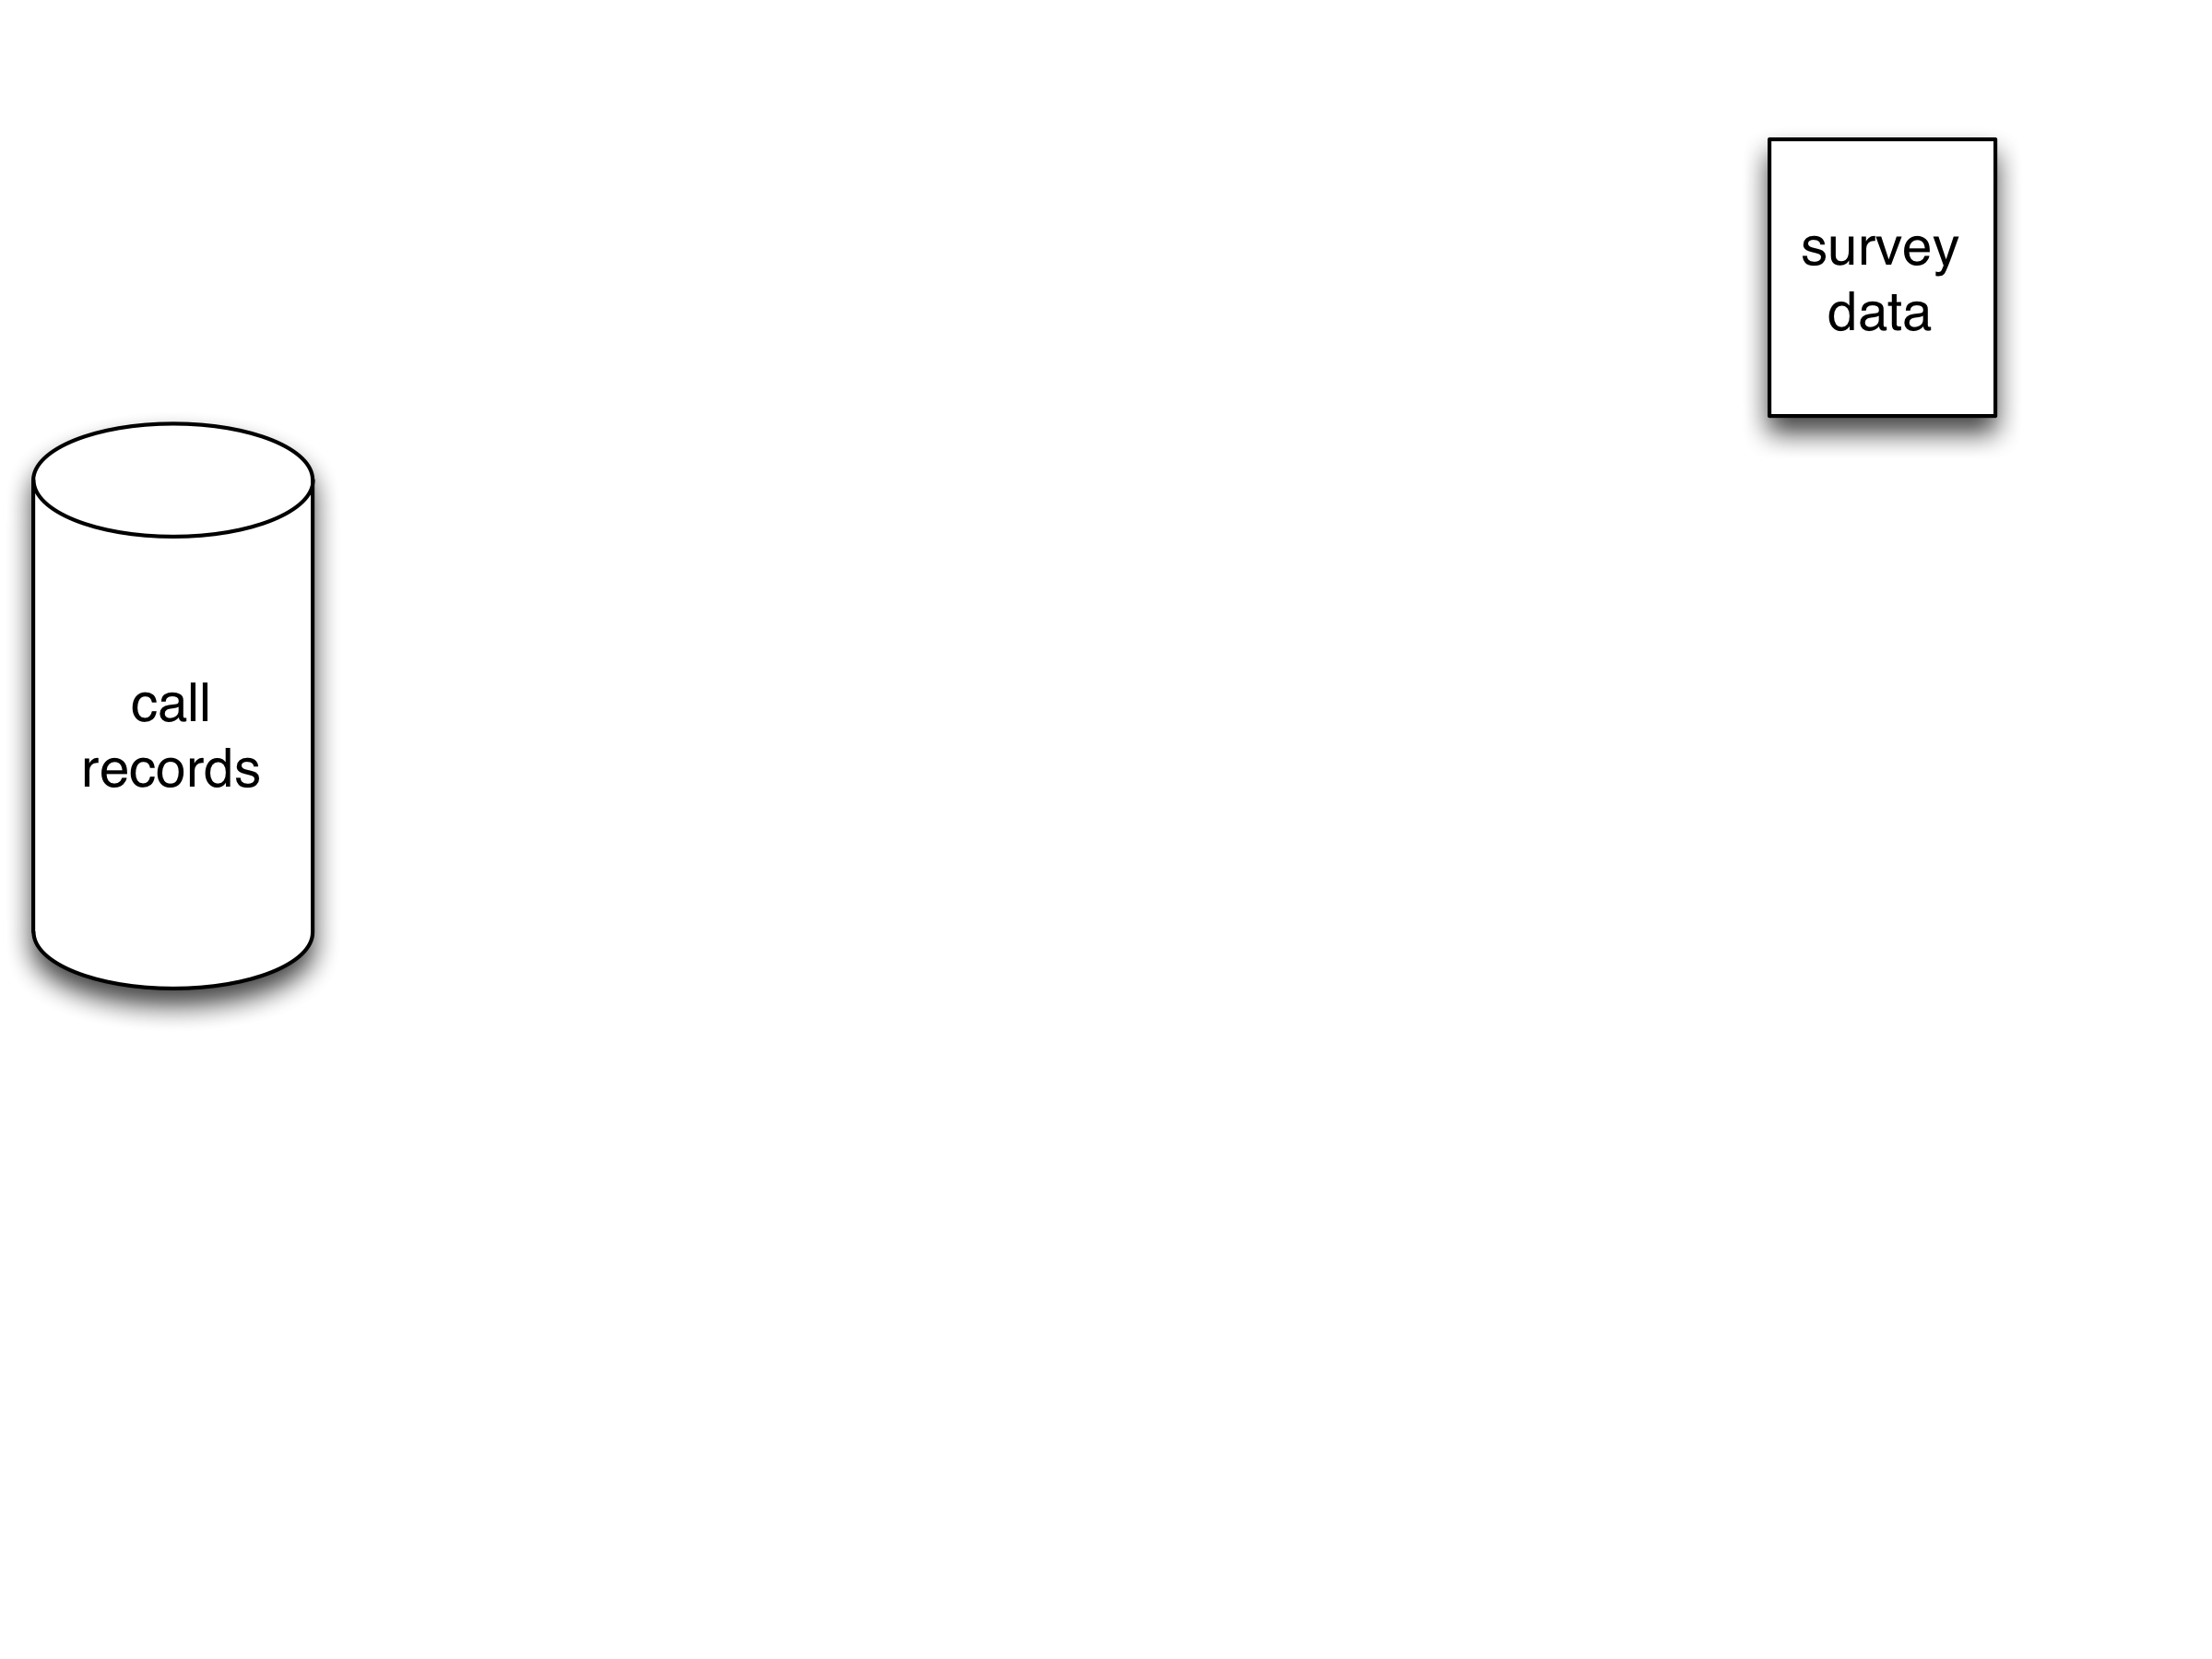
\includegraphics[width=0.7\textwidth]{figures/blumenstock_predicting_2015_schematic_2}}
\only<3>{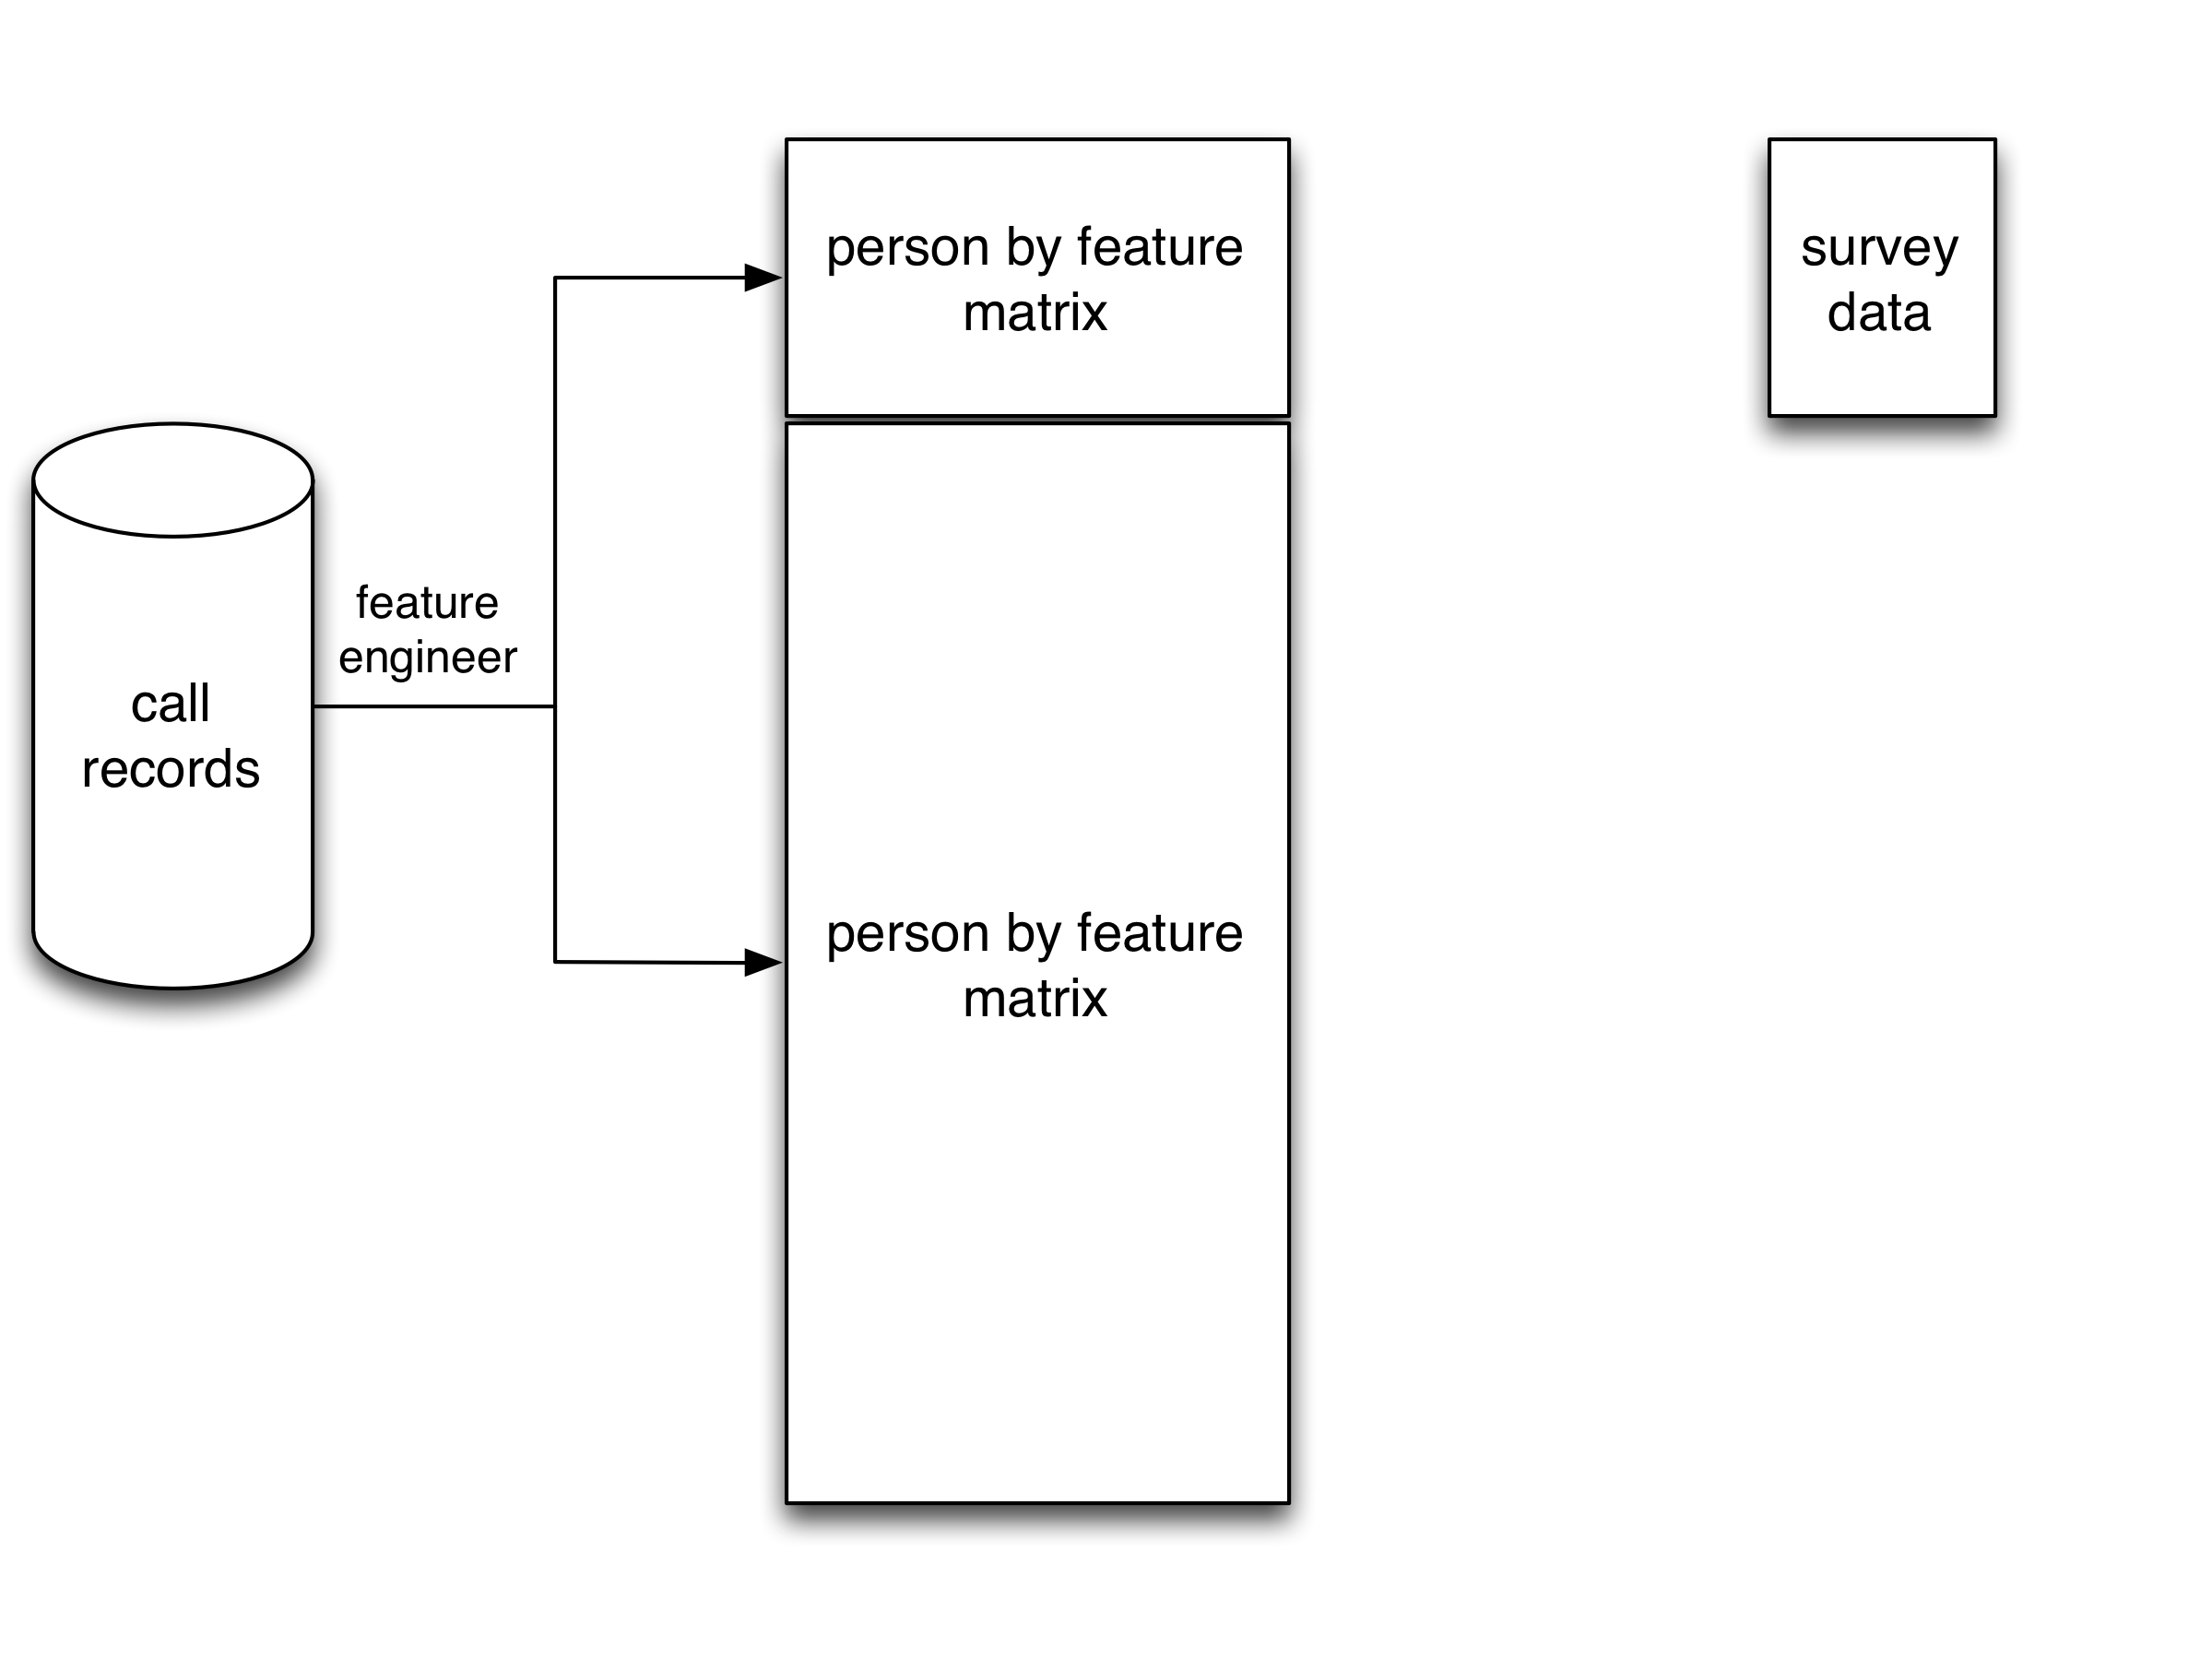
\includegraphics[width=0.7\textwidth]{figures/blumenstock_predicting_2015_schematic_3}}
\only<4>{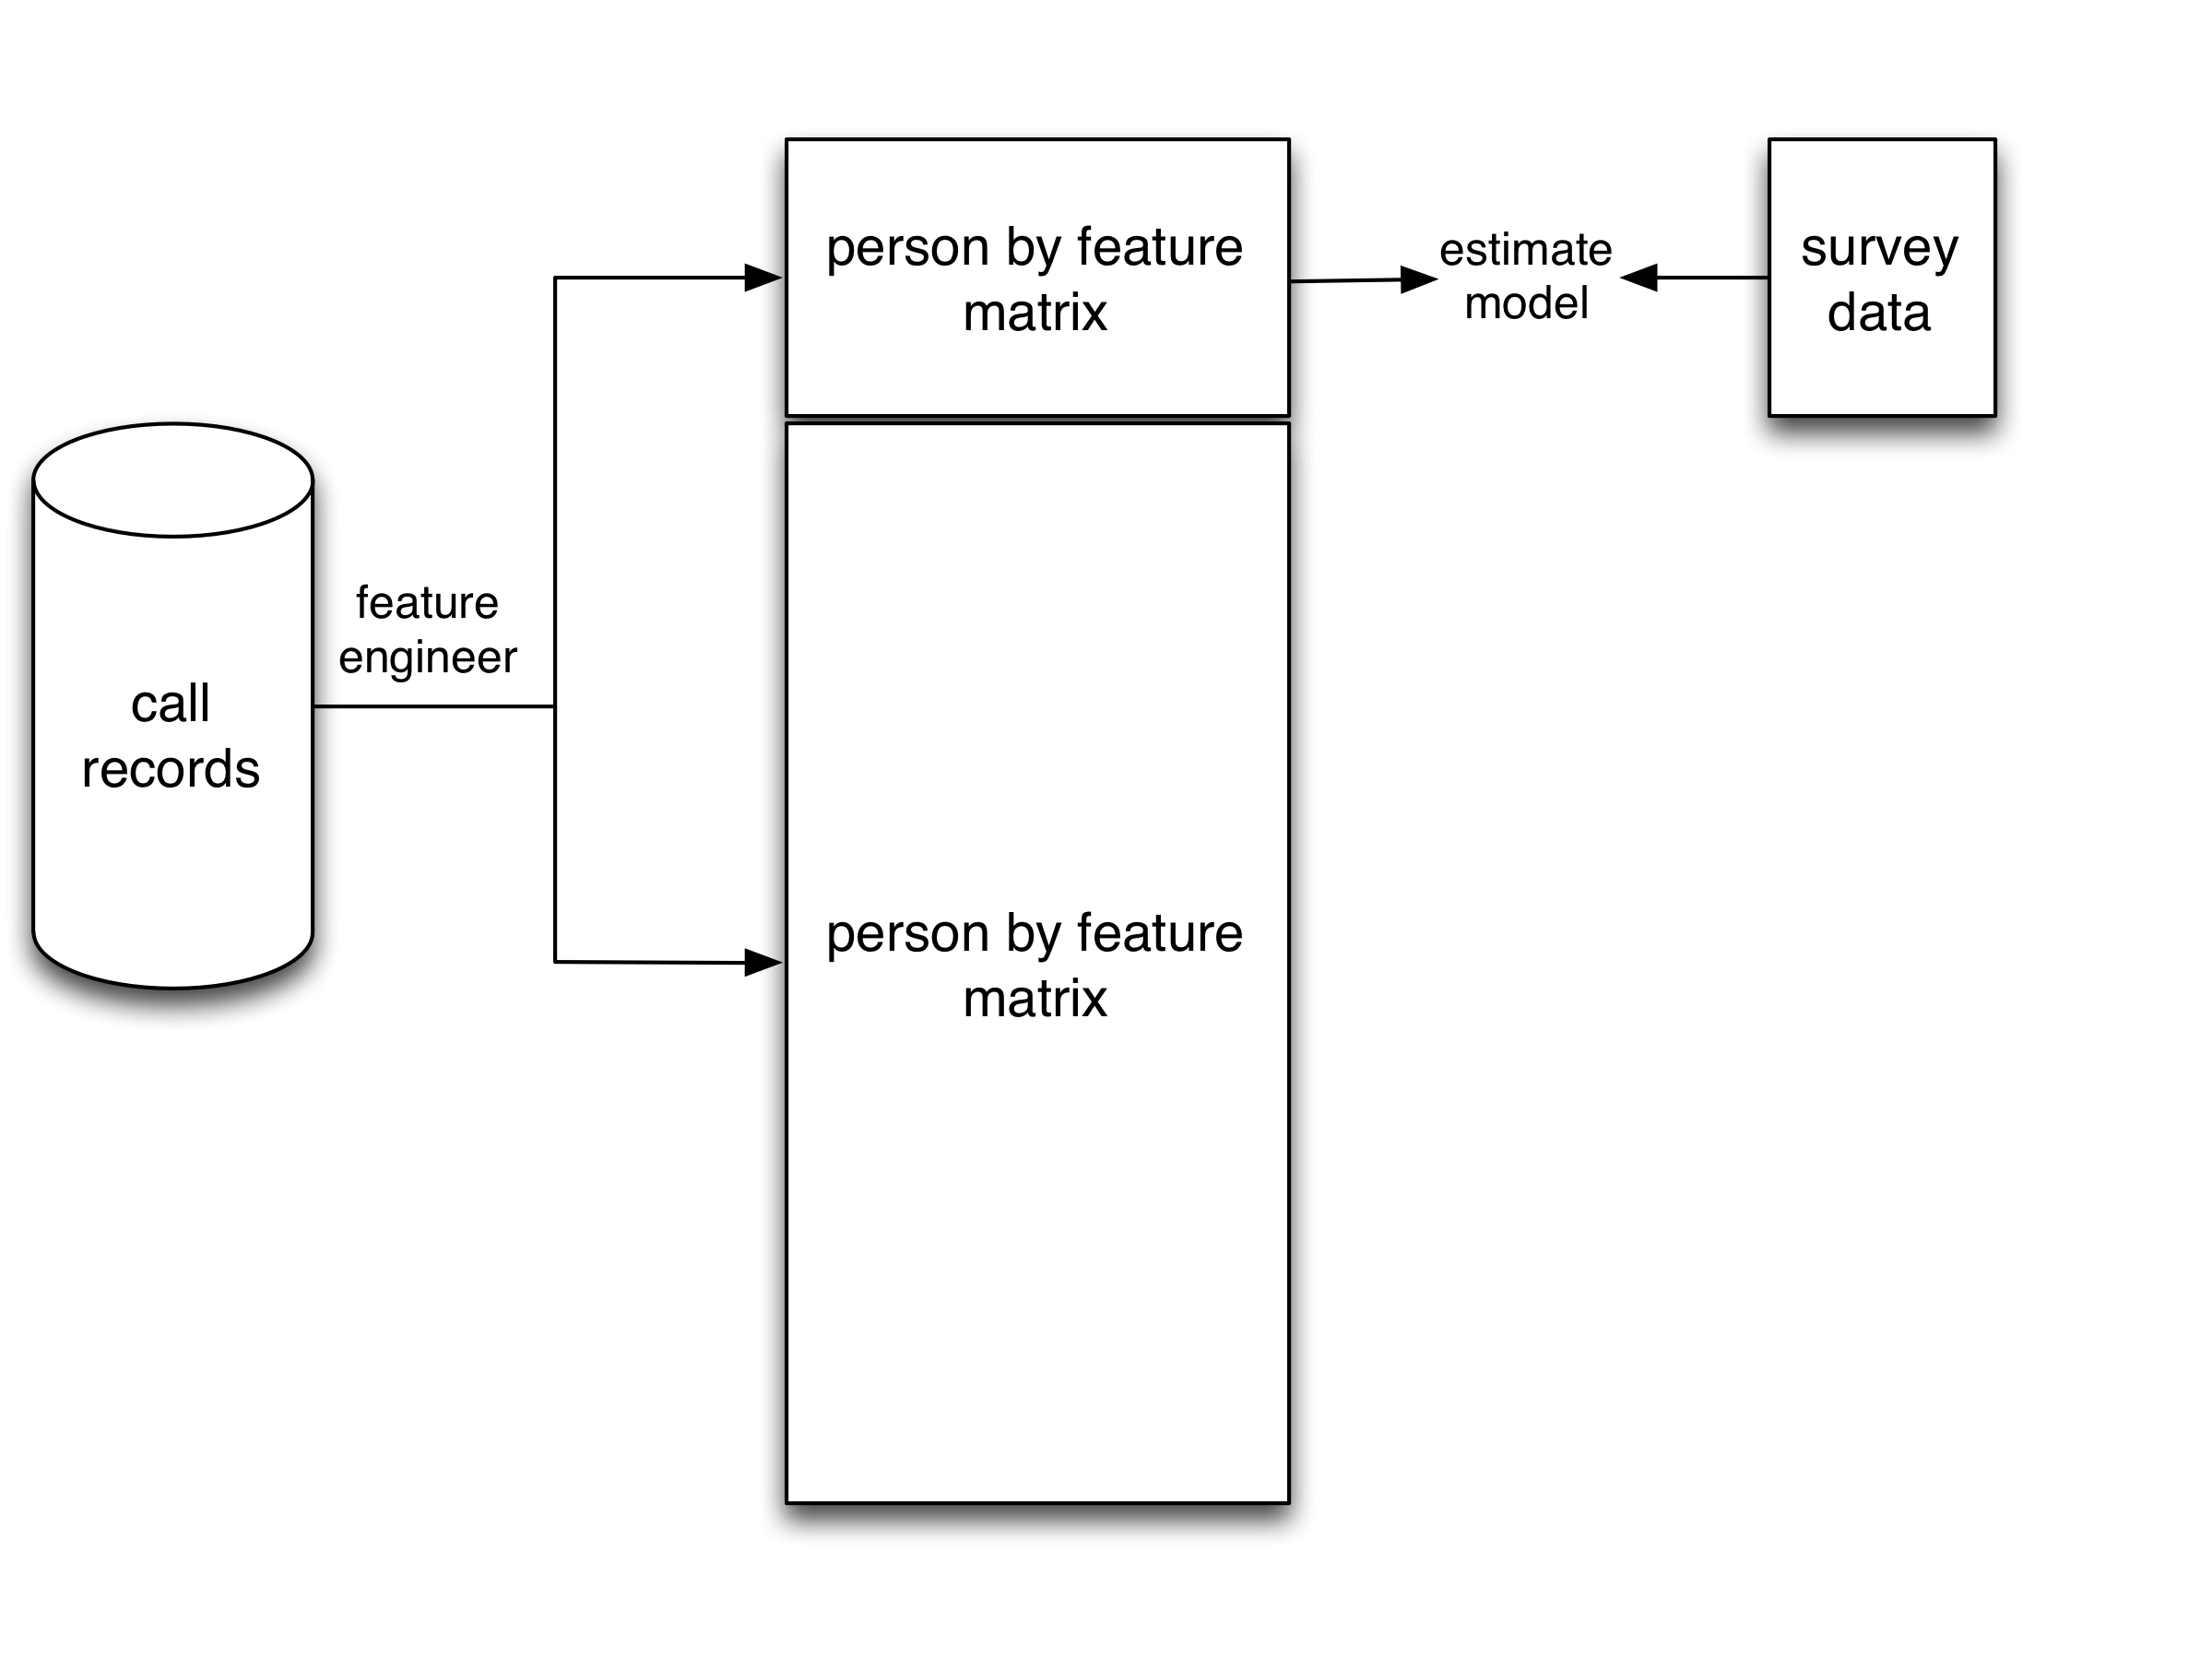
\includegraphics[width=0.7\textwidth]{figures/blumenstock_predicting_2015_schematic_4}}
\only<5>{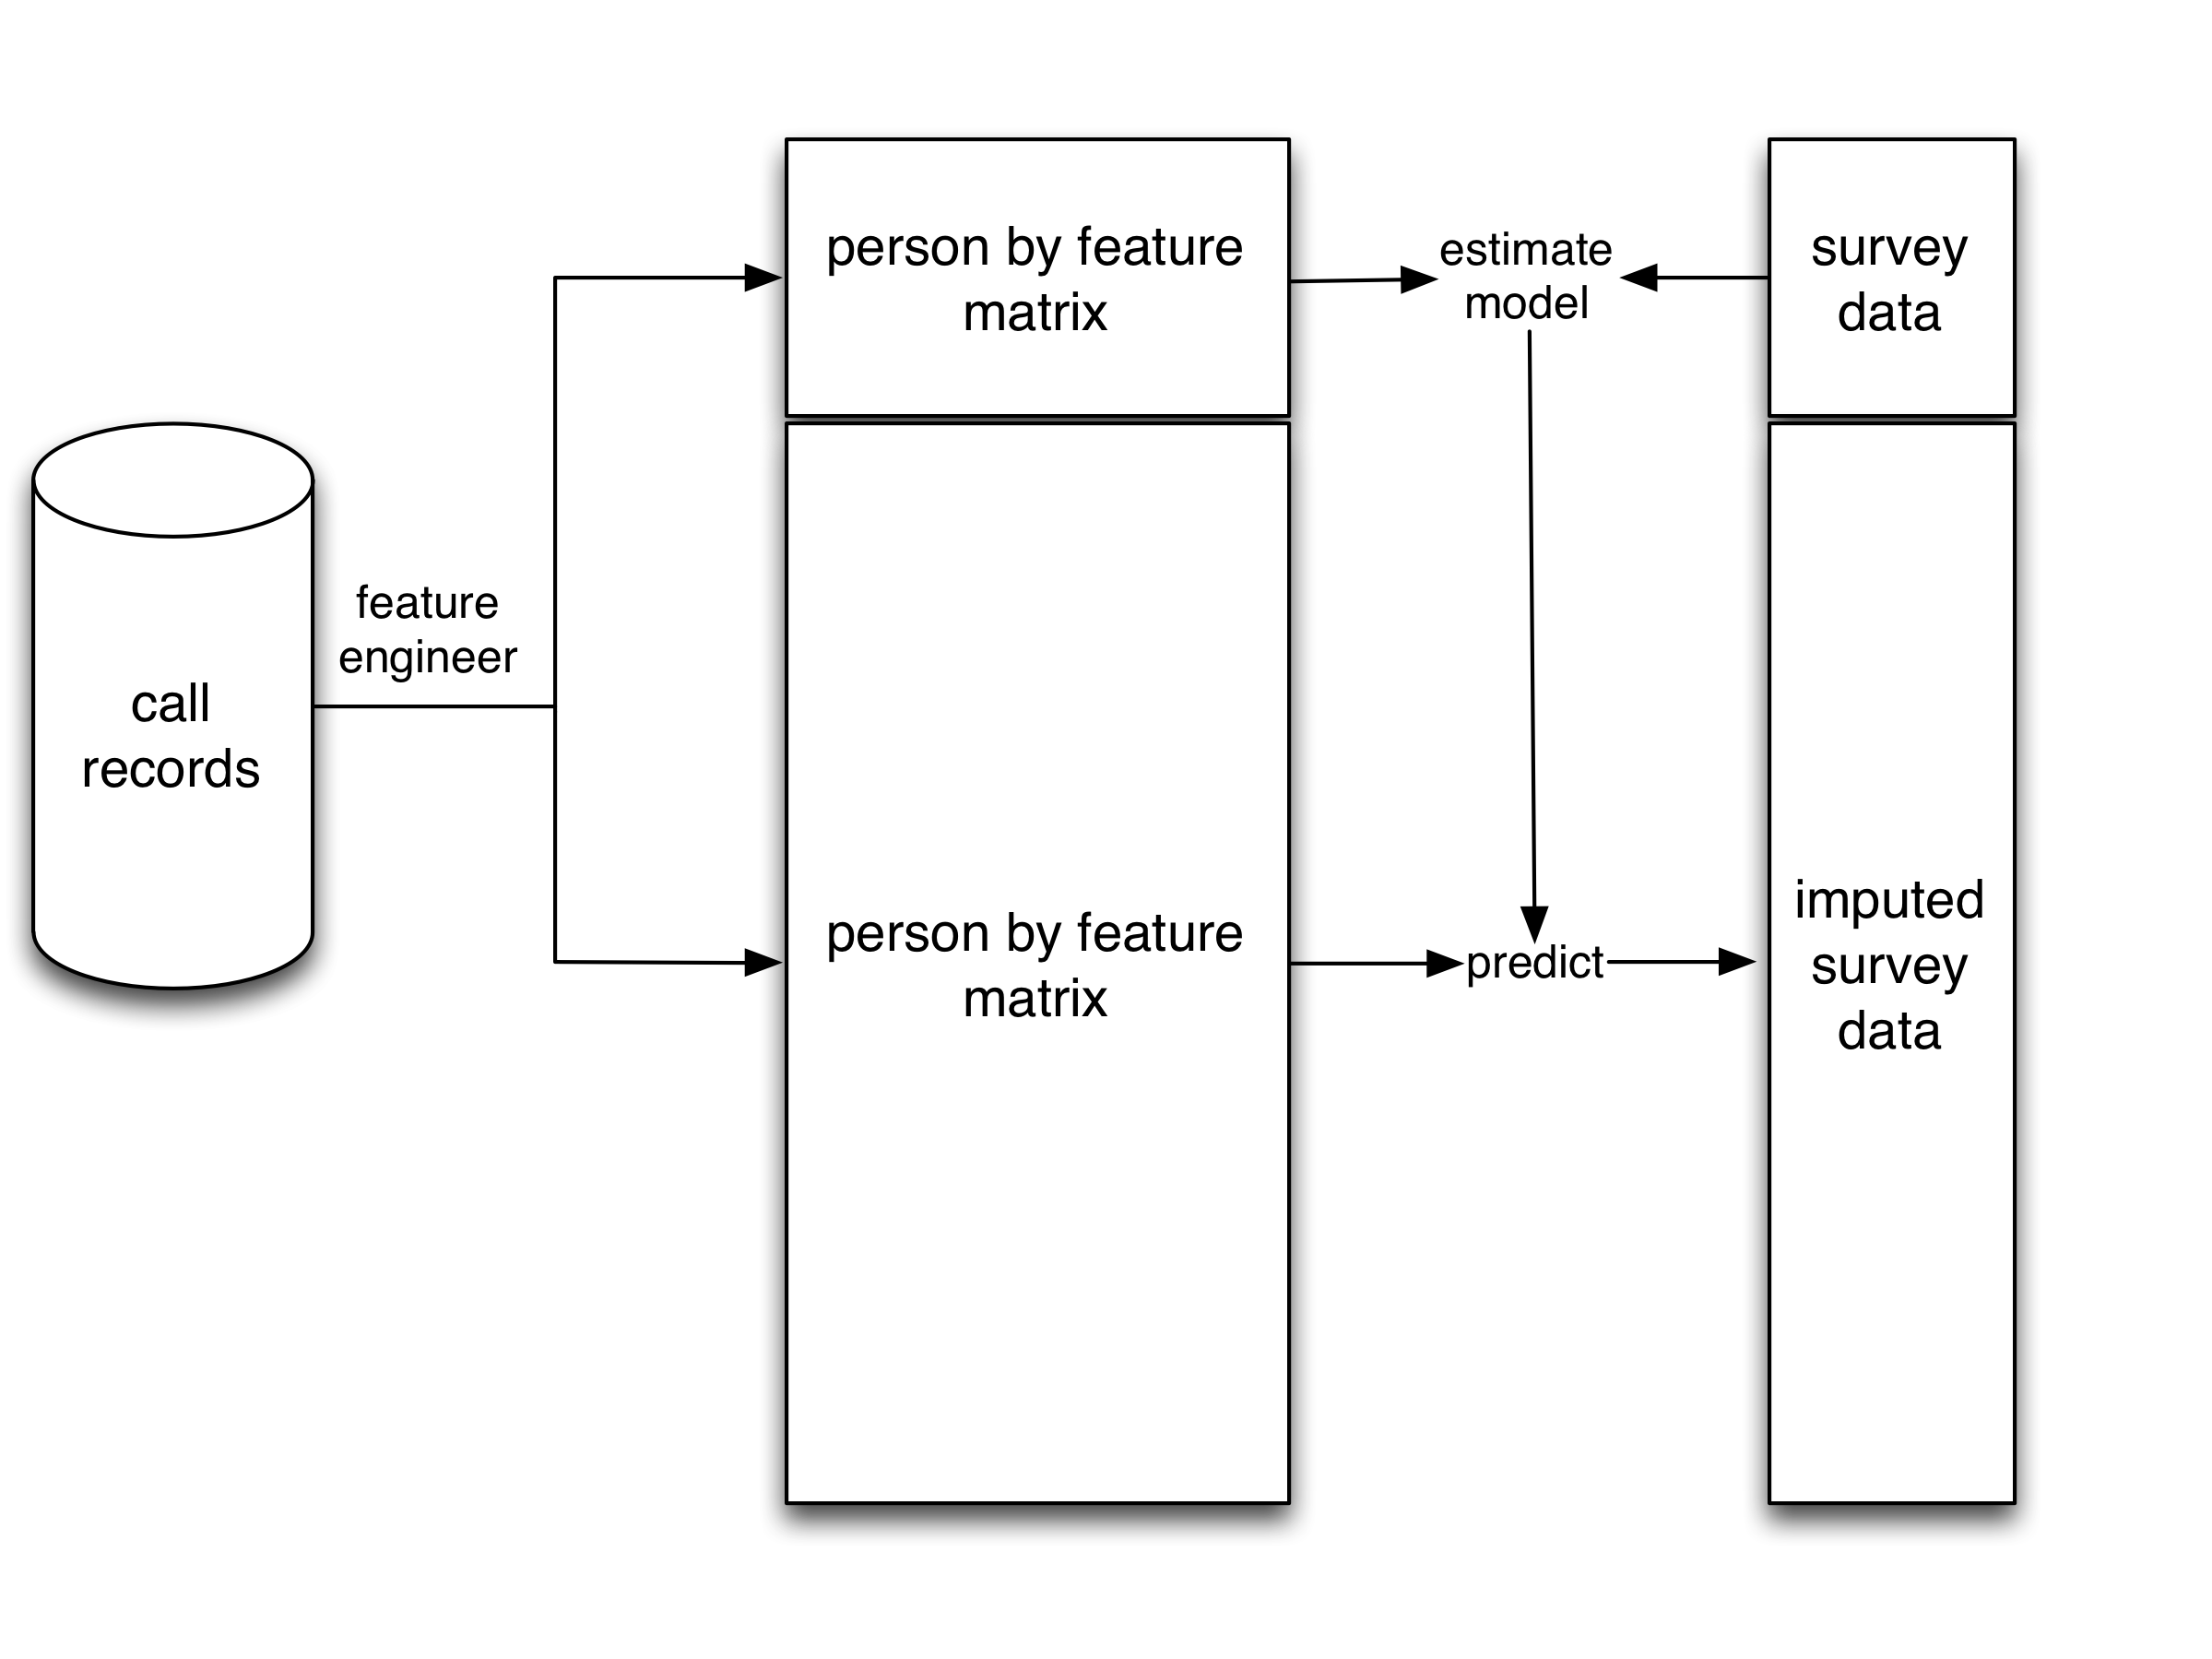
\includegraphics[width=0.7\textwidth]{figures/blumenstock_predicting_2015_schematic_5}}
\only<6>{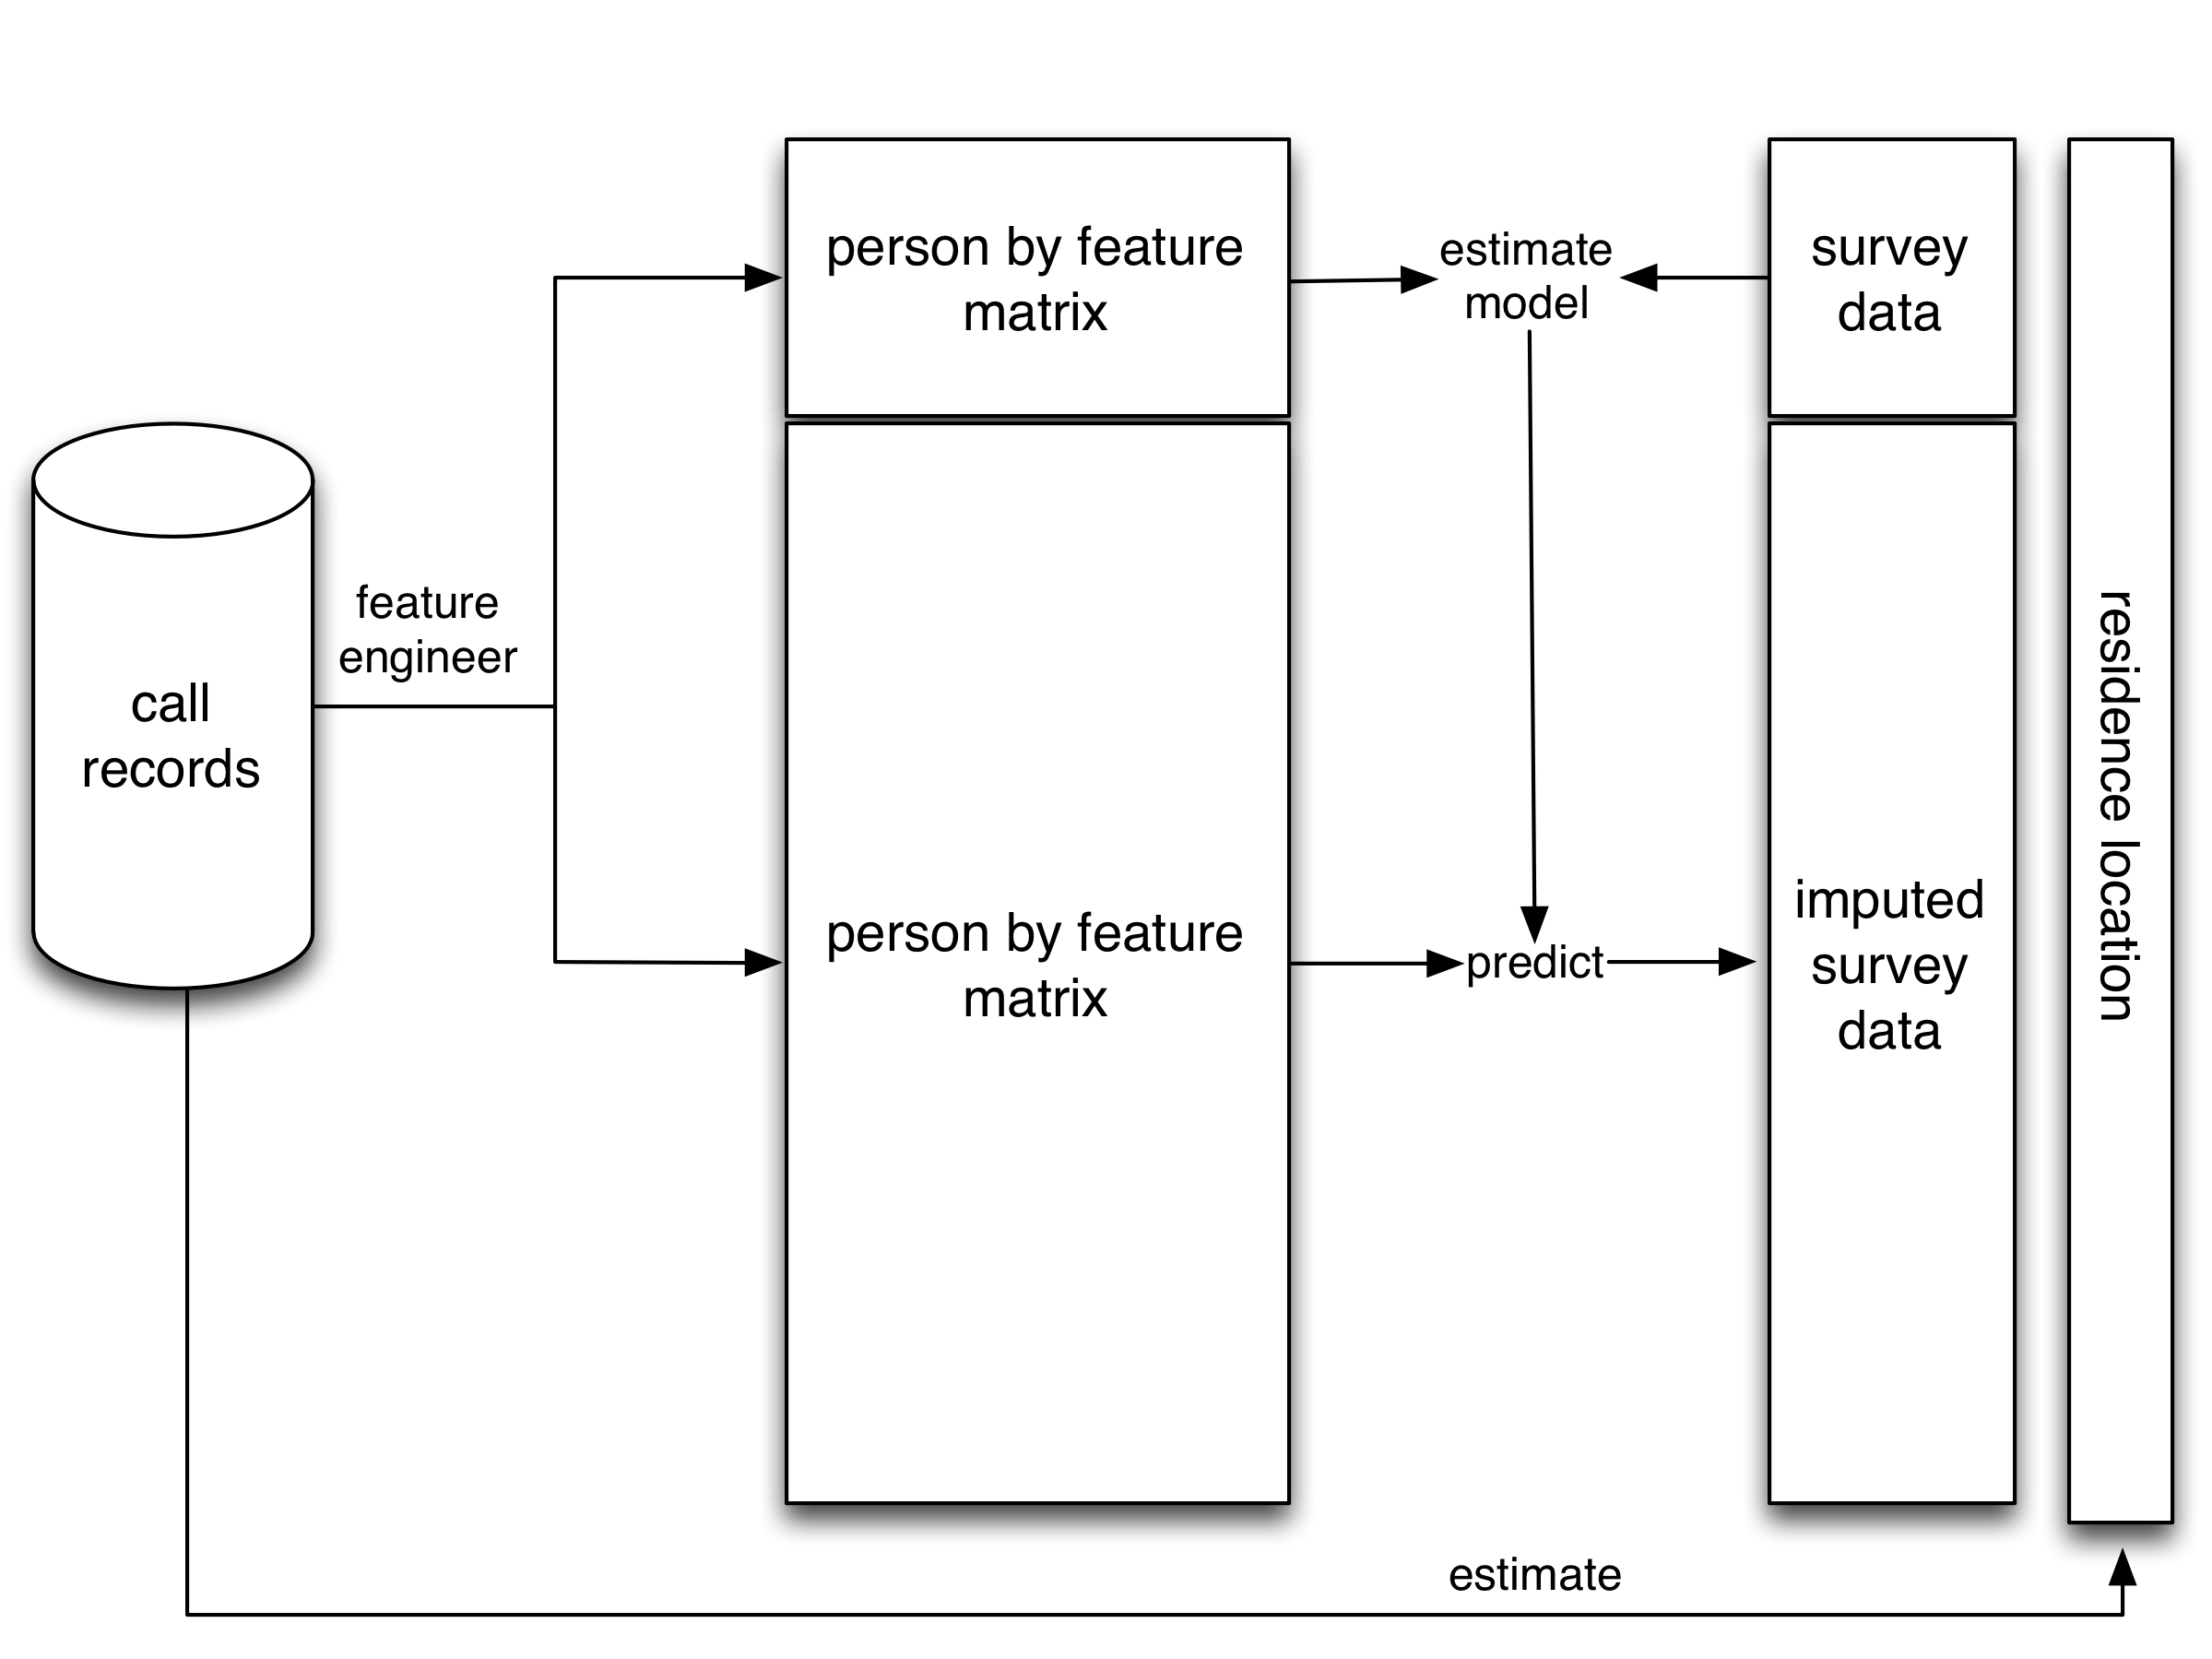
\includegraphics[width=0.7\textwidth]{figures/blumenstock_predicting_2015_schematic_6}}
\end{center}

\end{frame}
%%%%%%%%%%%%%%%%%%%%%%%%%%%
\begin{frame}

\begin{center}
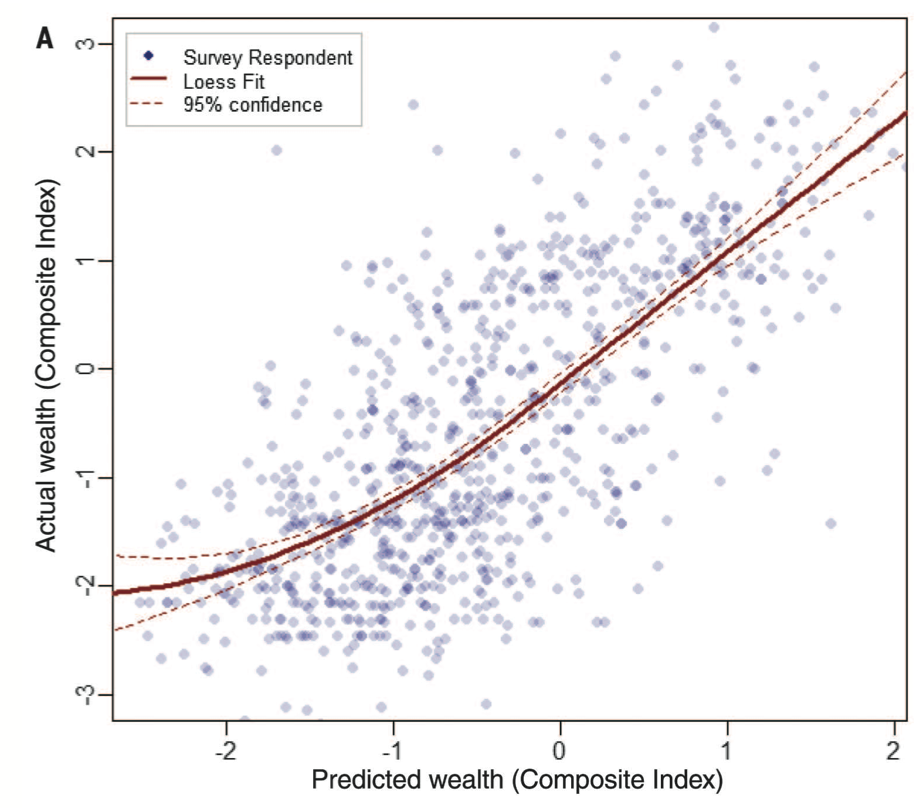
\includegraphics[width=0.7\textwidth]{figures/blumenstock_predicting_2015_fig1a}
\end{center}

\end{frame}
%%%%%%%%%%%%%%%%%%%%%%%%%%
\begin{frame}

\begin{center}
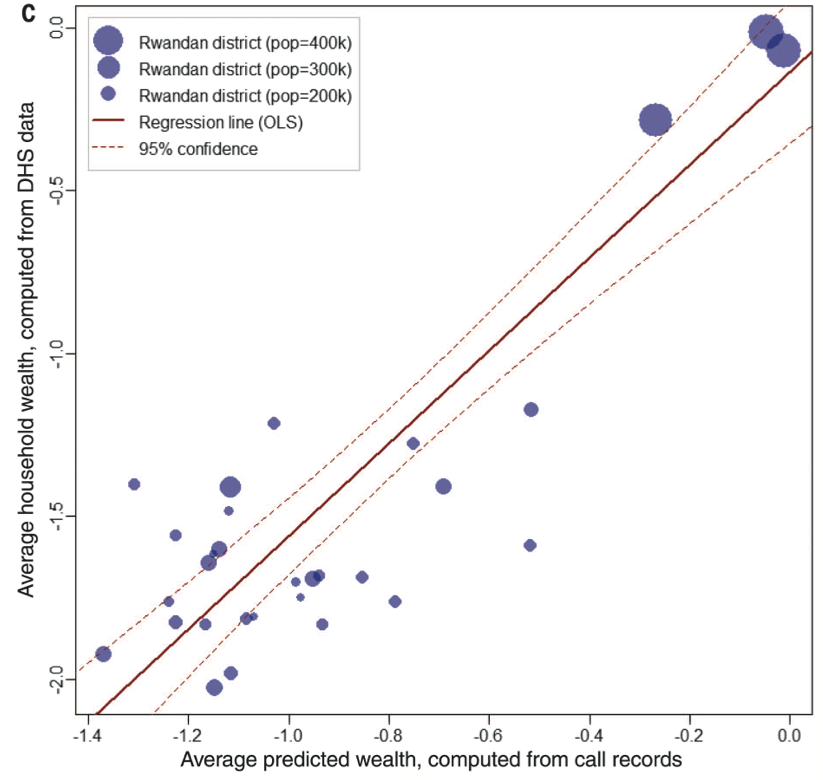
\includegraphics[width=0.45\textwidth]{figures/blumenstock_predicting_2015_fig3c}
\end{center}

\pause

\begin{itemize}
\item 10 times faster
\item 50 times cheaper
\end{itemize}

\end{frame}
%%%%%%%%%%%%%%%%%%%%%%%%%%
\begin{frame}

\begin{center}
\begin{tabular}{ccc}
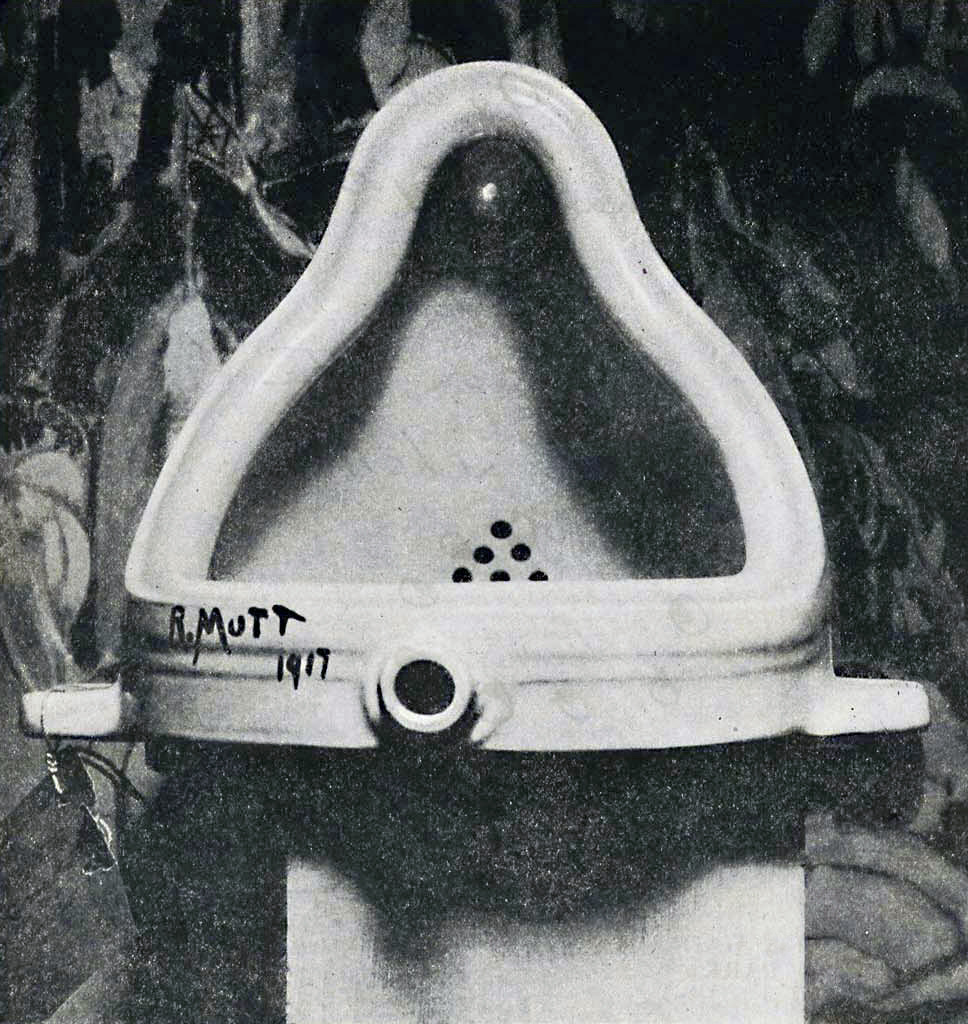
\includegraphics[width=0.30\textwidth]{figures/duchamp_fountain} & \phantom{12} \LARGE{+} \phantom{12} & 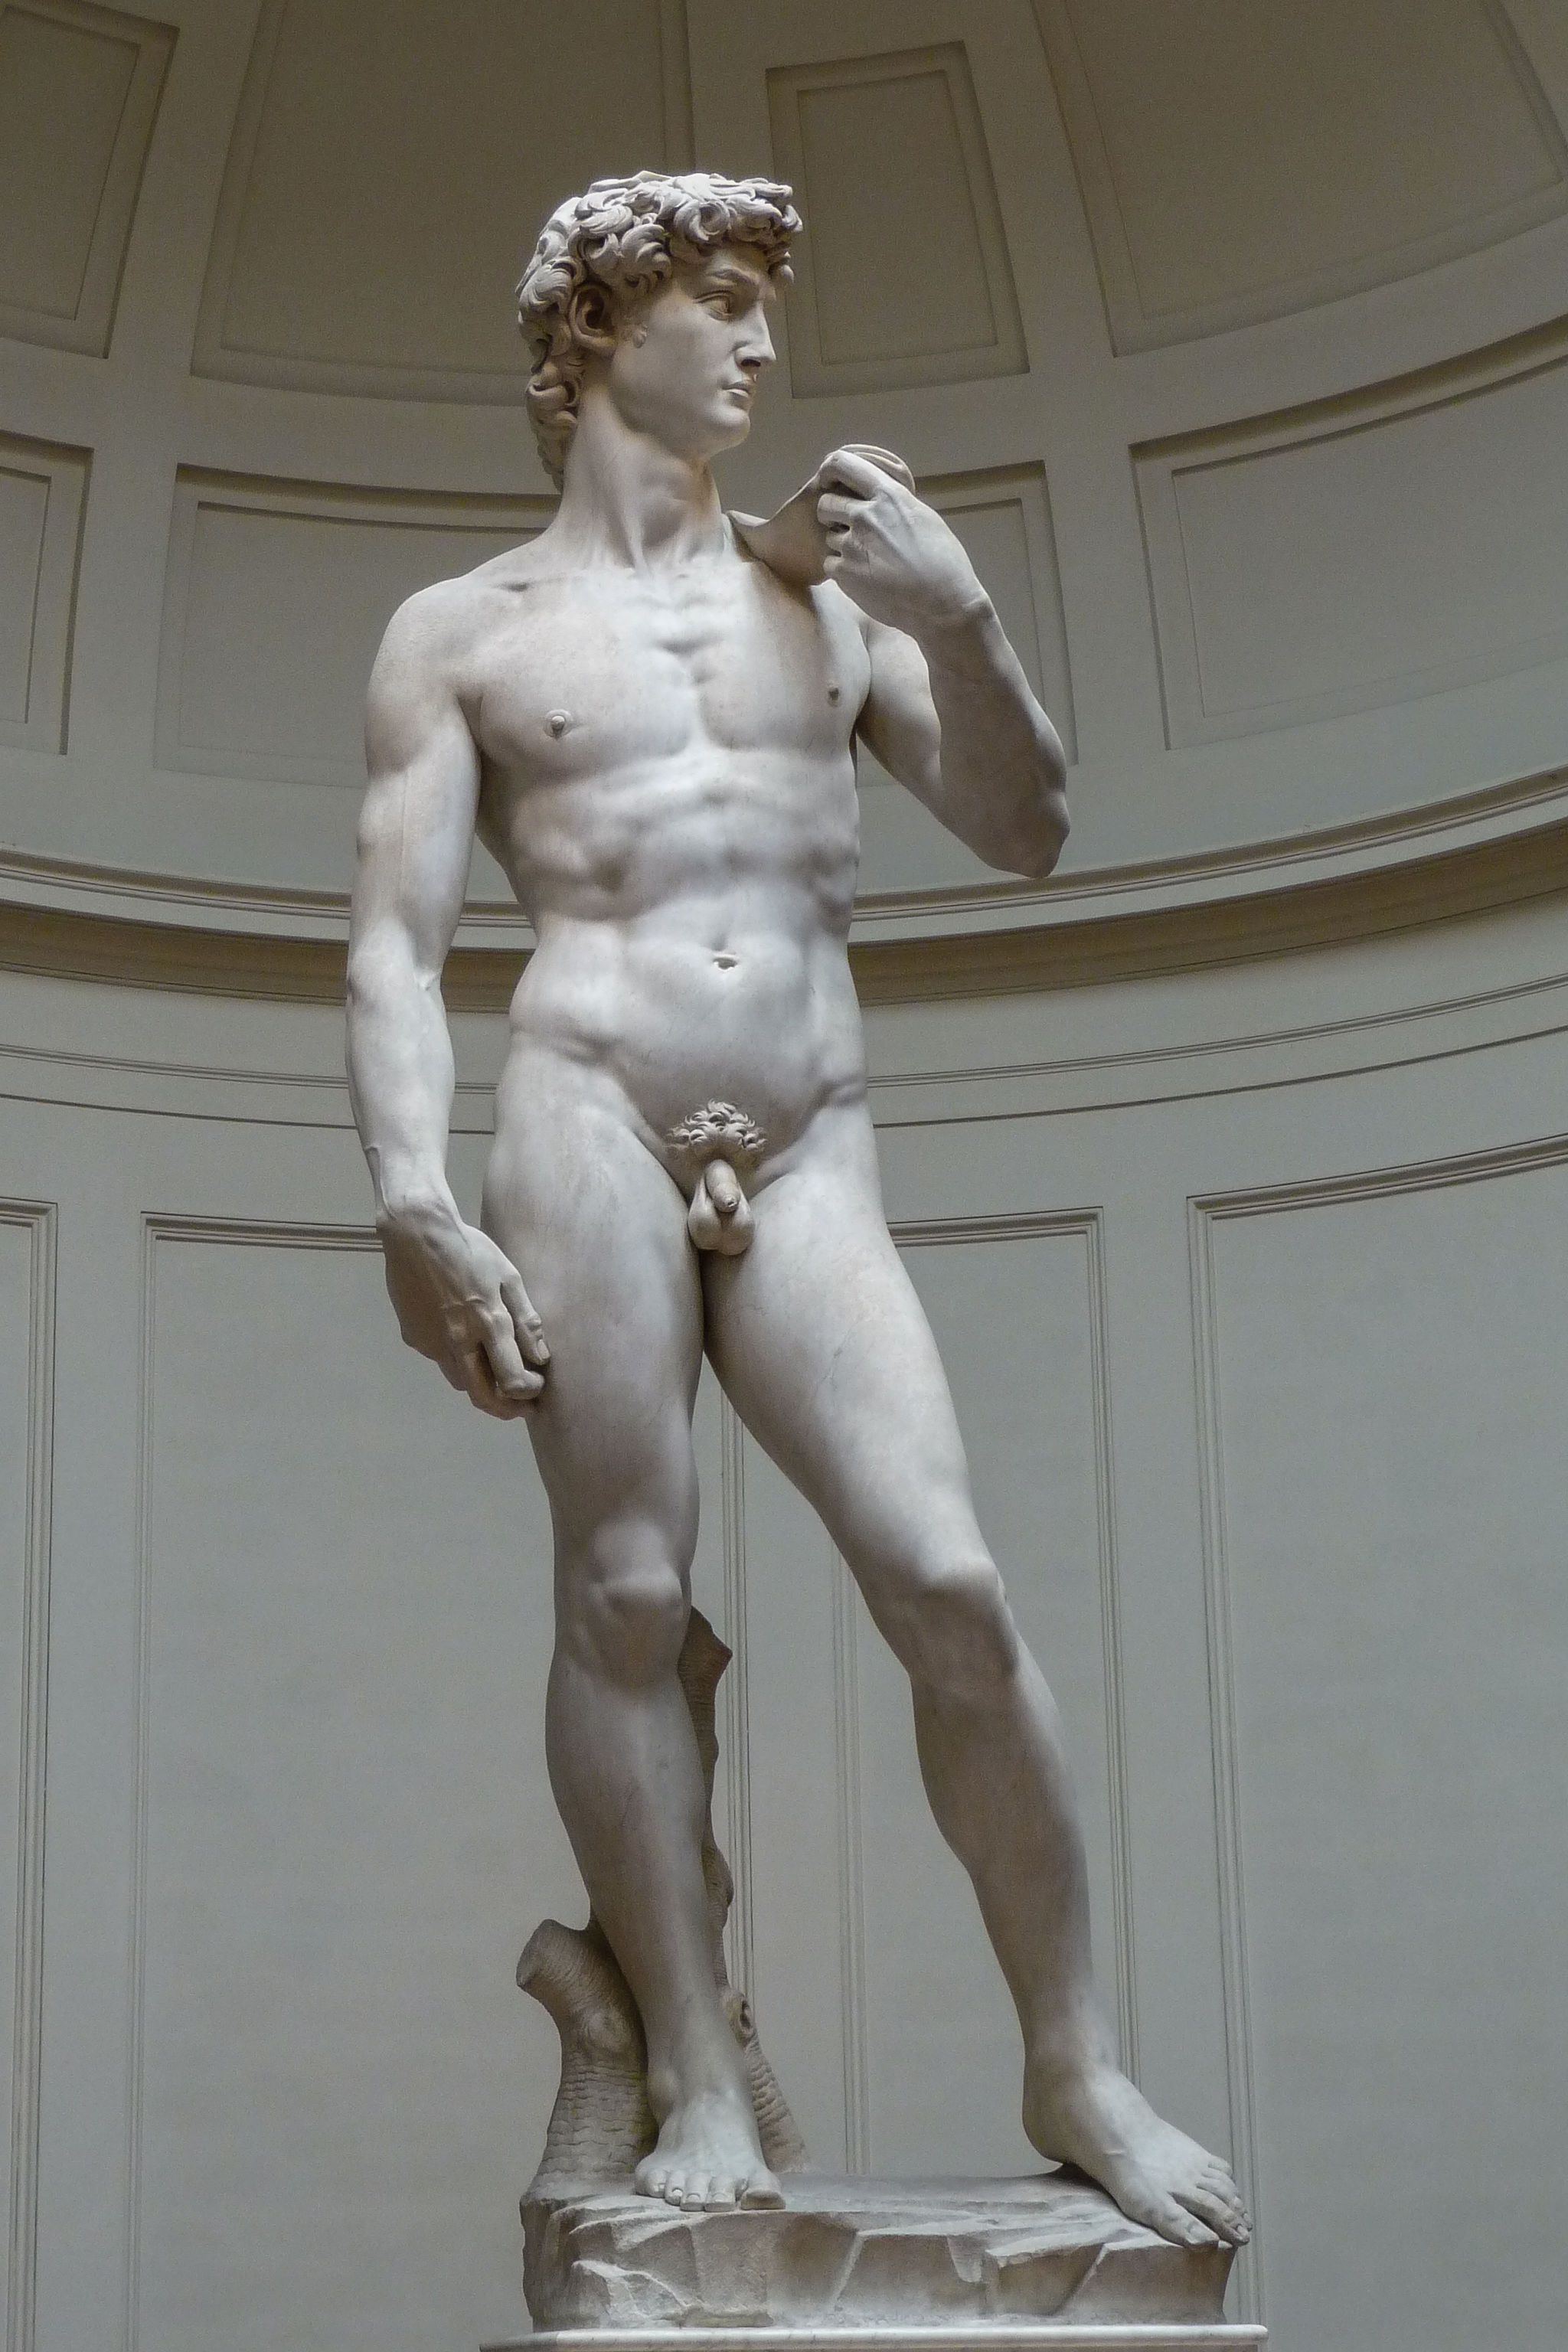
\includegraphics[width=0.30\textwidth]{figures/michelangelo_david} \\
\LARGE{Readymades} &  & \LARGE{Custommades}
\end{tabular}
\end{center}

\vf
\vspace{0.2in}
\TINY{\url{https://commons.wikimedia.org/wiki/File:Duchamp_Fountaine.jpg}}\\
\TINY{\url{https://commons.wikimedia.org/wiki/File:\%27David\%27_by_Michelangelo_JBU0001.JPG}}

\end{frame}
%%%%%%%%%%%%%%%%%%%%%%%%%%%
\begin{frame}

\begin{center}
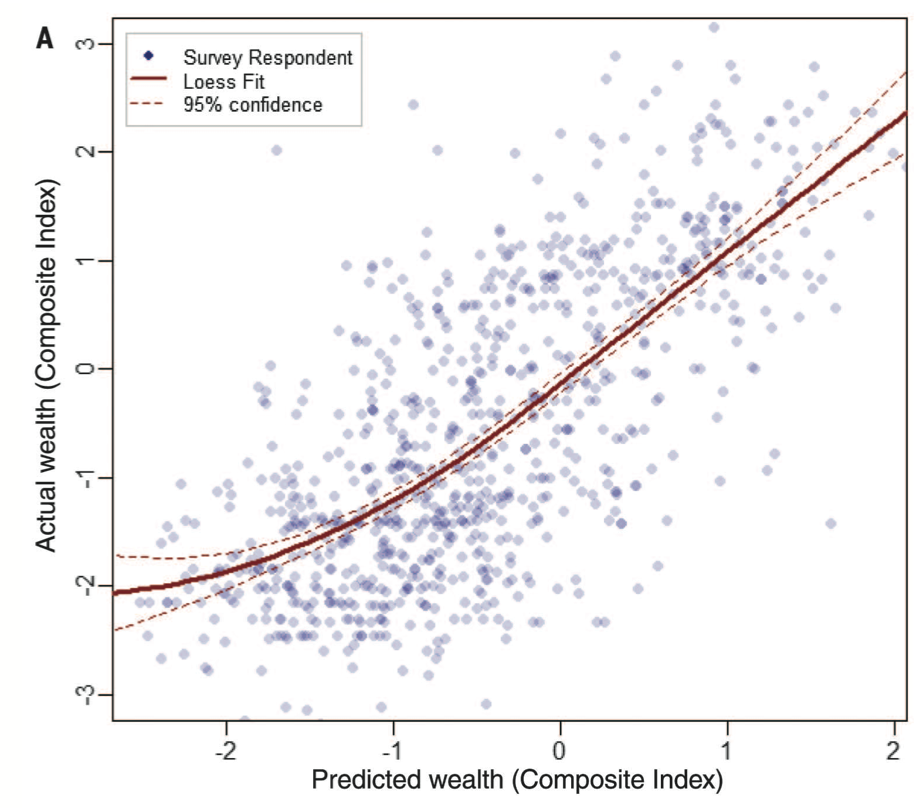
\includegraphics[width=0.4\textwidth]{figures/blumenstock_predicting_2015_fig1a}
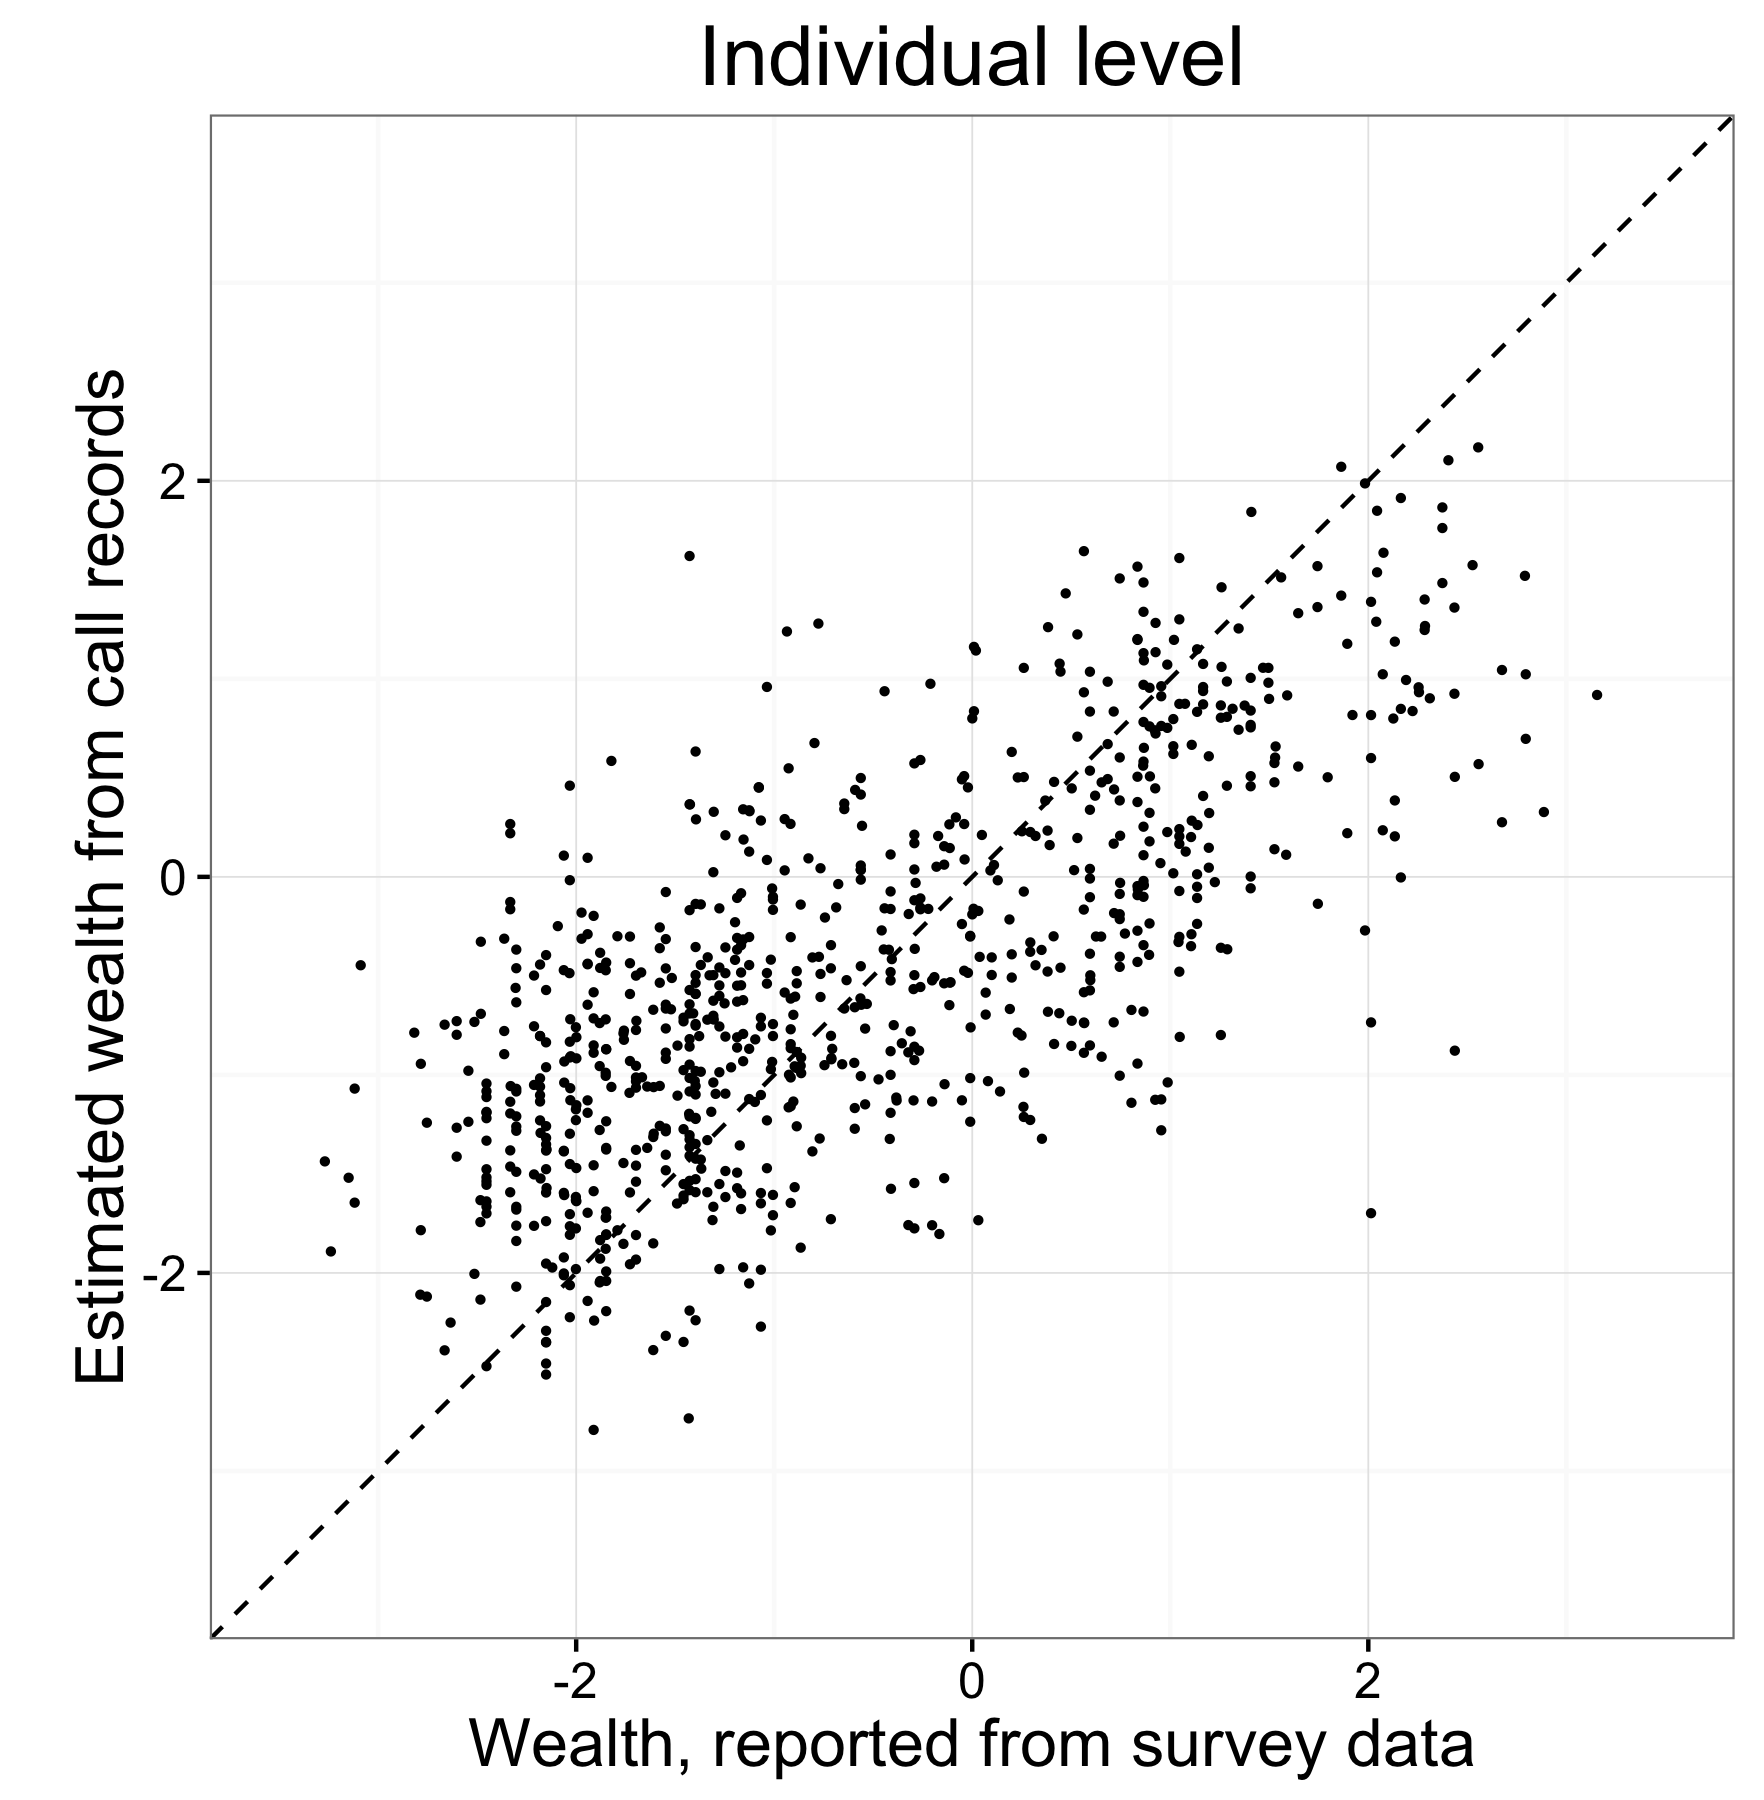
\includegraphics[width=0.4\textwidth]{figures/blumenstock_predicting_2015_fig1a_replotted}
\end{center}

\end{frame}
%%%%%%%%%%%%%%%%%%%%%%%%%%
\begin{frame}

\begin{center}
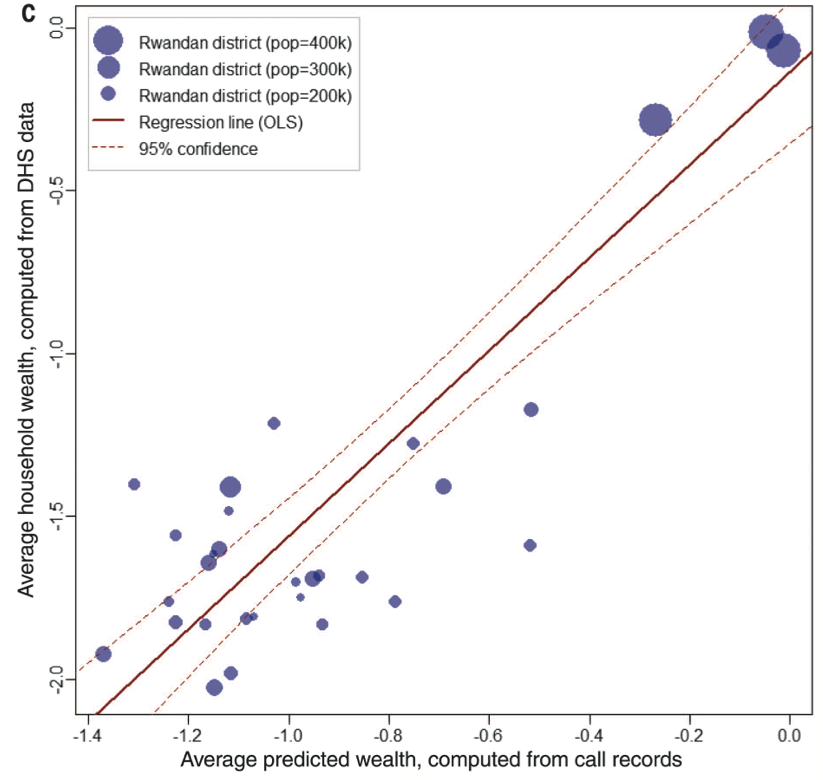
\includegraphics[width=0.4\textwidth]{figures/blumenstock_predicting_2015_fig3c}
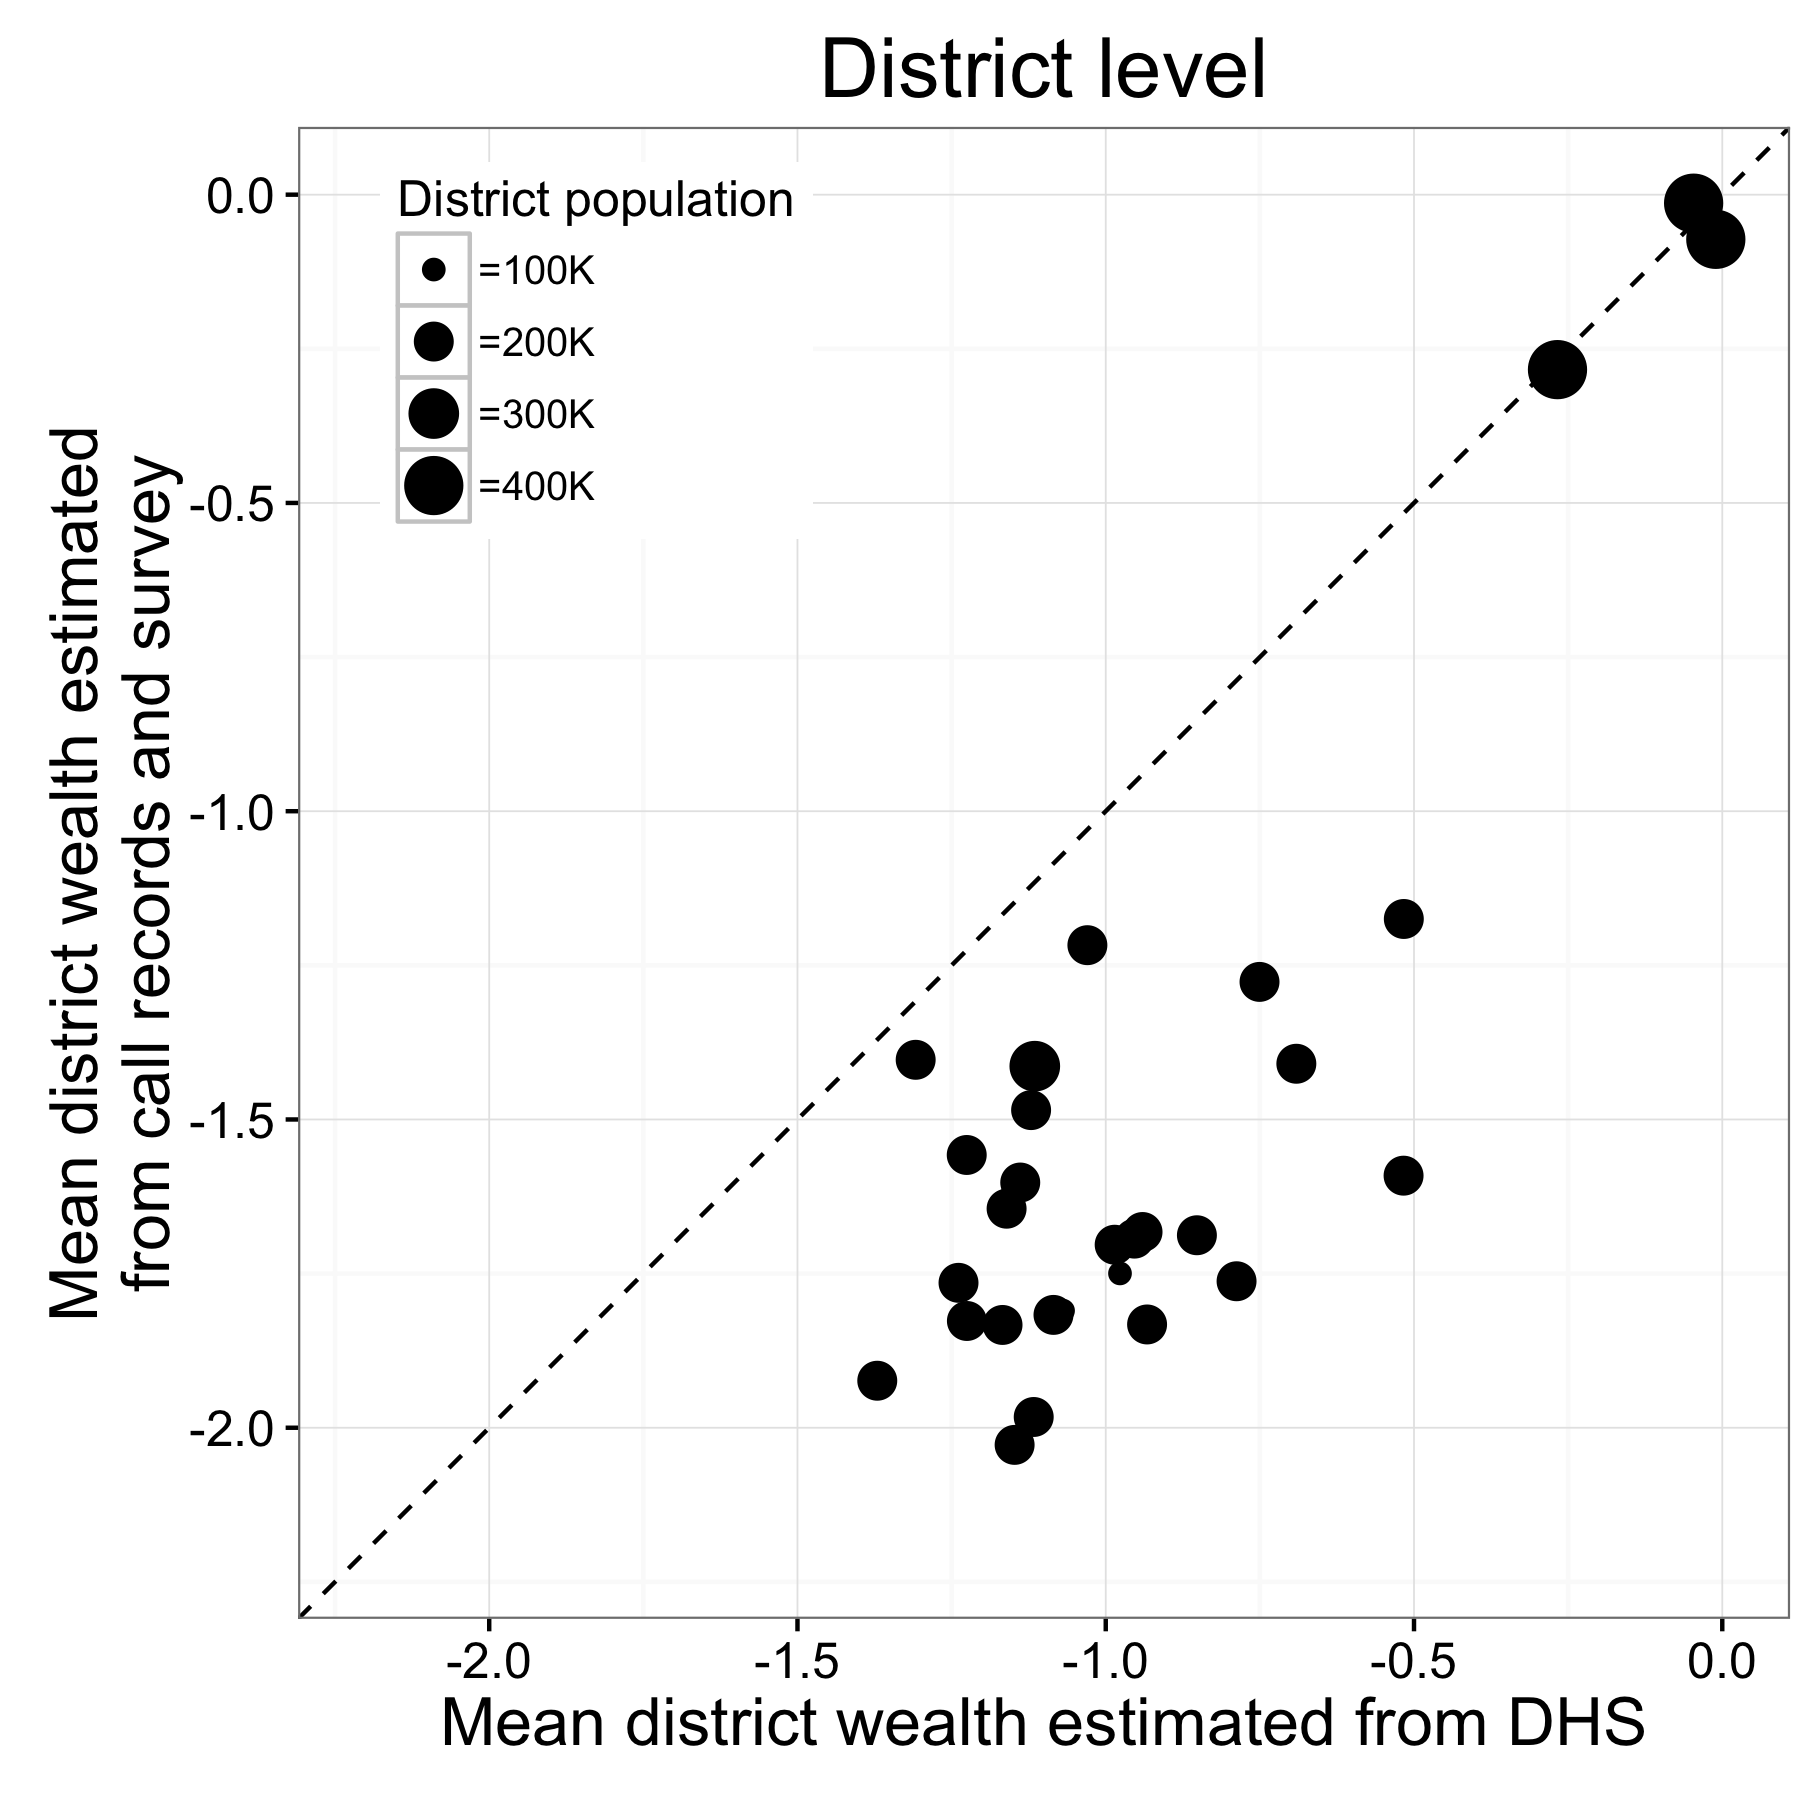
\includegraphics[width=0.4\textwidth]{figures/blumenstock_predicting_2015_fig3c_replotted}
\end{center}

\end{frame}
%%%%%%%%%%%%%%%%%%%%%%%%%%
\begin{frame}

\begin{center}
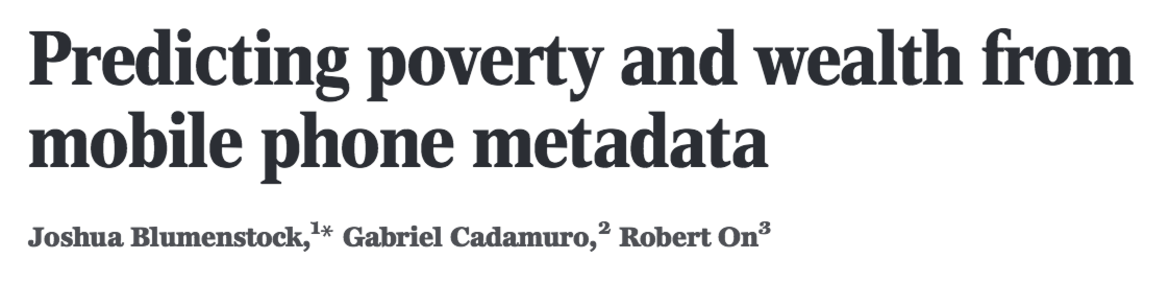
\includegraphics[width=0.3\textwidth]{figures/blumenstock_predicting_2015_title}
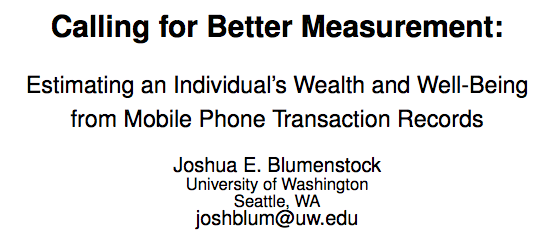
\includegraphics[width=0.3\textwidth]{figures/blumenstock_calling_2014_title}
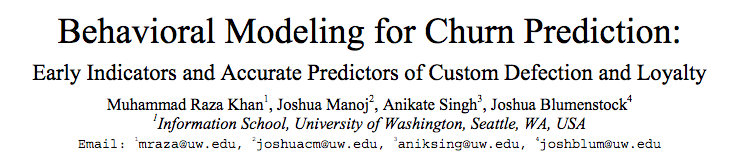
\includegraphics[width=0.3\textwidth]{figures/khan_behavioral_2015_title}
\end{center}

\end{frame}
%%%%%%%%%%%%%%%%%%%%%%%%%%
\begin{frame}

\begin{center}
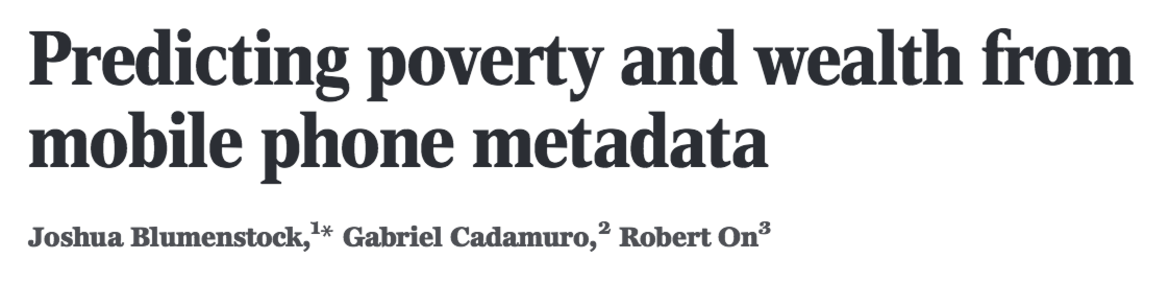
\includegraphics[width=0.4\textwidth]{figures/blumenstock_predicting_2015_title}
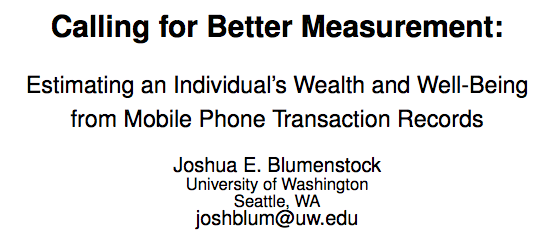
\includegraphics[width=0.4\textwidth]{figures/blumenstock_calling_2014_title}
\end{center}

\pause
\begin{itemize}
\item better feature engineering
\item new outcome variable
\item out-of-sample test
\end{itemize}

\end{frame}
%%%%%%%%%%%%%%%%%%%%%%%%%%
\begin{frame}

\begin{center}
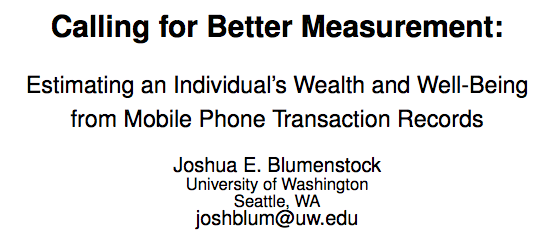
\includegraphics[width=0.4\textwidth]{figures/blumenstock_calling_2014_title}
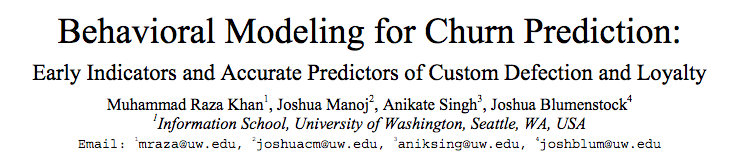
\includegraphics[width=0.4\textwidth]{figures/khan_behavioral_2015_title}
\end{center}

\pause
\begin{itemize}
\item outcome in data vs collected in a survey
\end{itemize}

\end{frame}
%%%%%%%%%%%%%%%%%%%%%%%%%%
\begin{frame}

\begin{center}
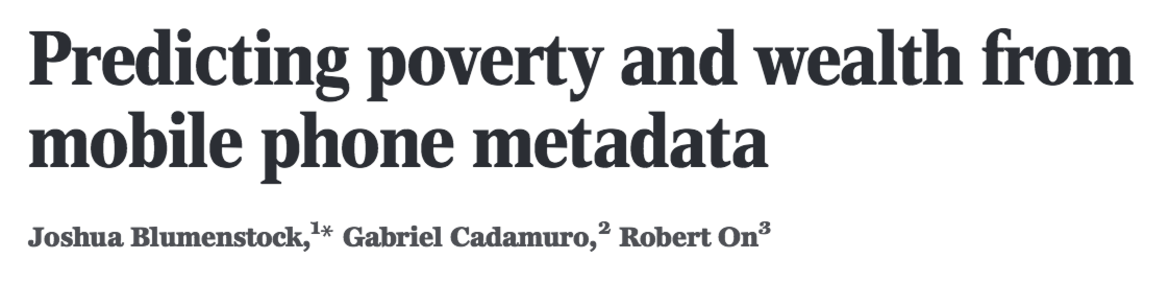
\includegraphics[width=0.4\textwidth]{figures/blumenstock_predicting_2015_title}
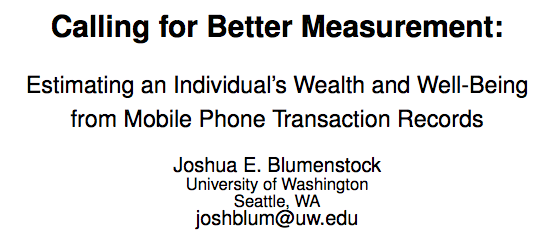
\includegraphics[width=0.4\textwidth]{figures/blumenstock_calling_2014_title}
\end{center}

\pause
\begin{itemize}
\item better feature engineering
\item new outcome variable
\item out-of-sample test
\end{itemize}

\end{frame}
%%%%%%%%%%%%%%%%%%%%%%%%%
\begin{frame}

\begin{center}
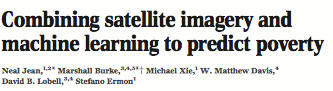
\includegraphics[width=0.8\textwidth]{figures/jean_combining_2016_title}
\end{center}

\vf

This paper is amazing and surprising.  First a digression . . . .

\end{frame}
%%%%%%%%%%%%%%%%%%%%%%%%
\begin{frame}

Supervised learning:\\
Lots of input-output pairs; goal is to develop a function that will predict the output from the input

\end{frame}
%%%%%%%%%%%%%%%%%%%%%%%%
\begin{frame}

\begin{center}
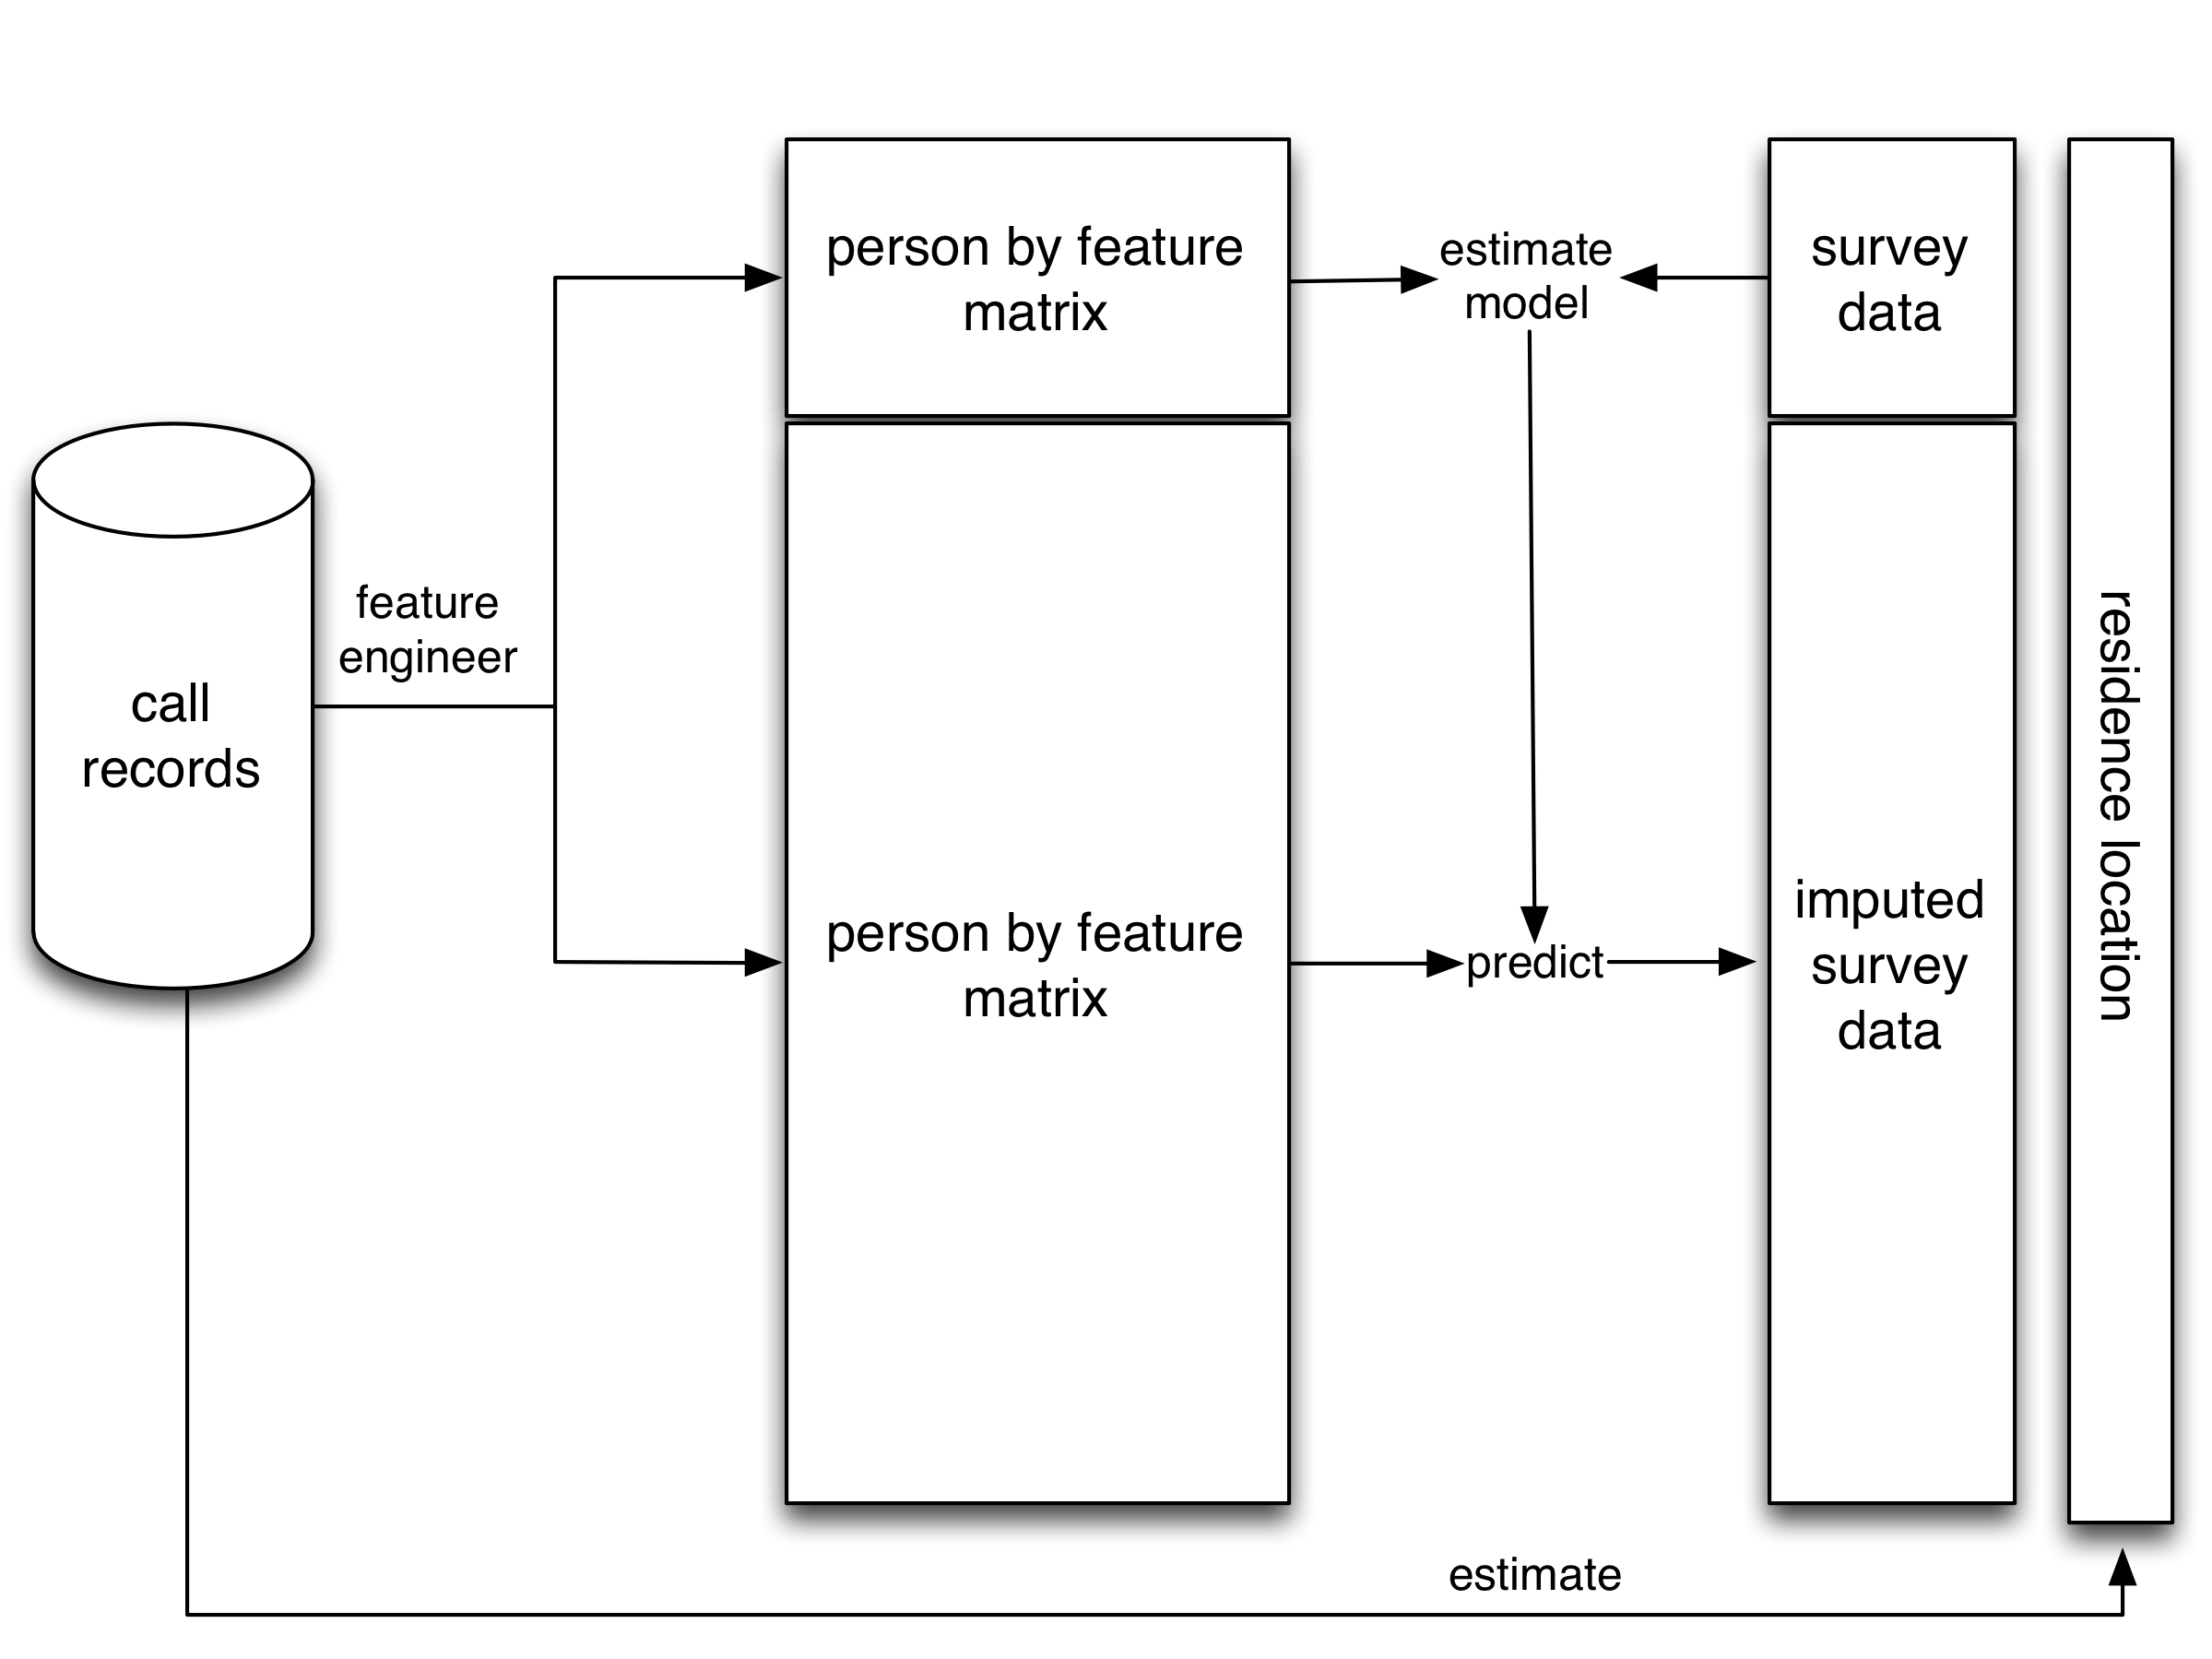
\includegraphics[width=0.7\textwidth]{figures/blumenstock_predicting_2015_schematic_6}
\end{center}
\vf
See Chapter 3 of Salganik (2016)
\end{frame}
%%%%%%%%%%%%%%%%%%%%%%%%%%%
\begin{frame}

\begin{center}
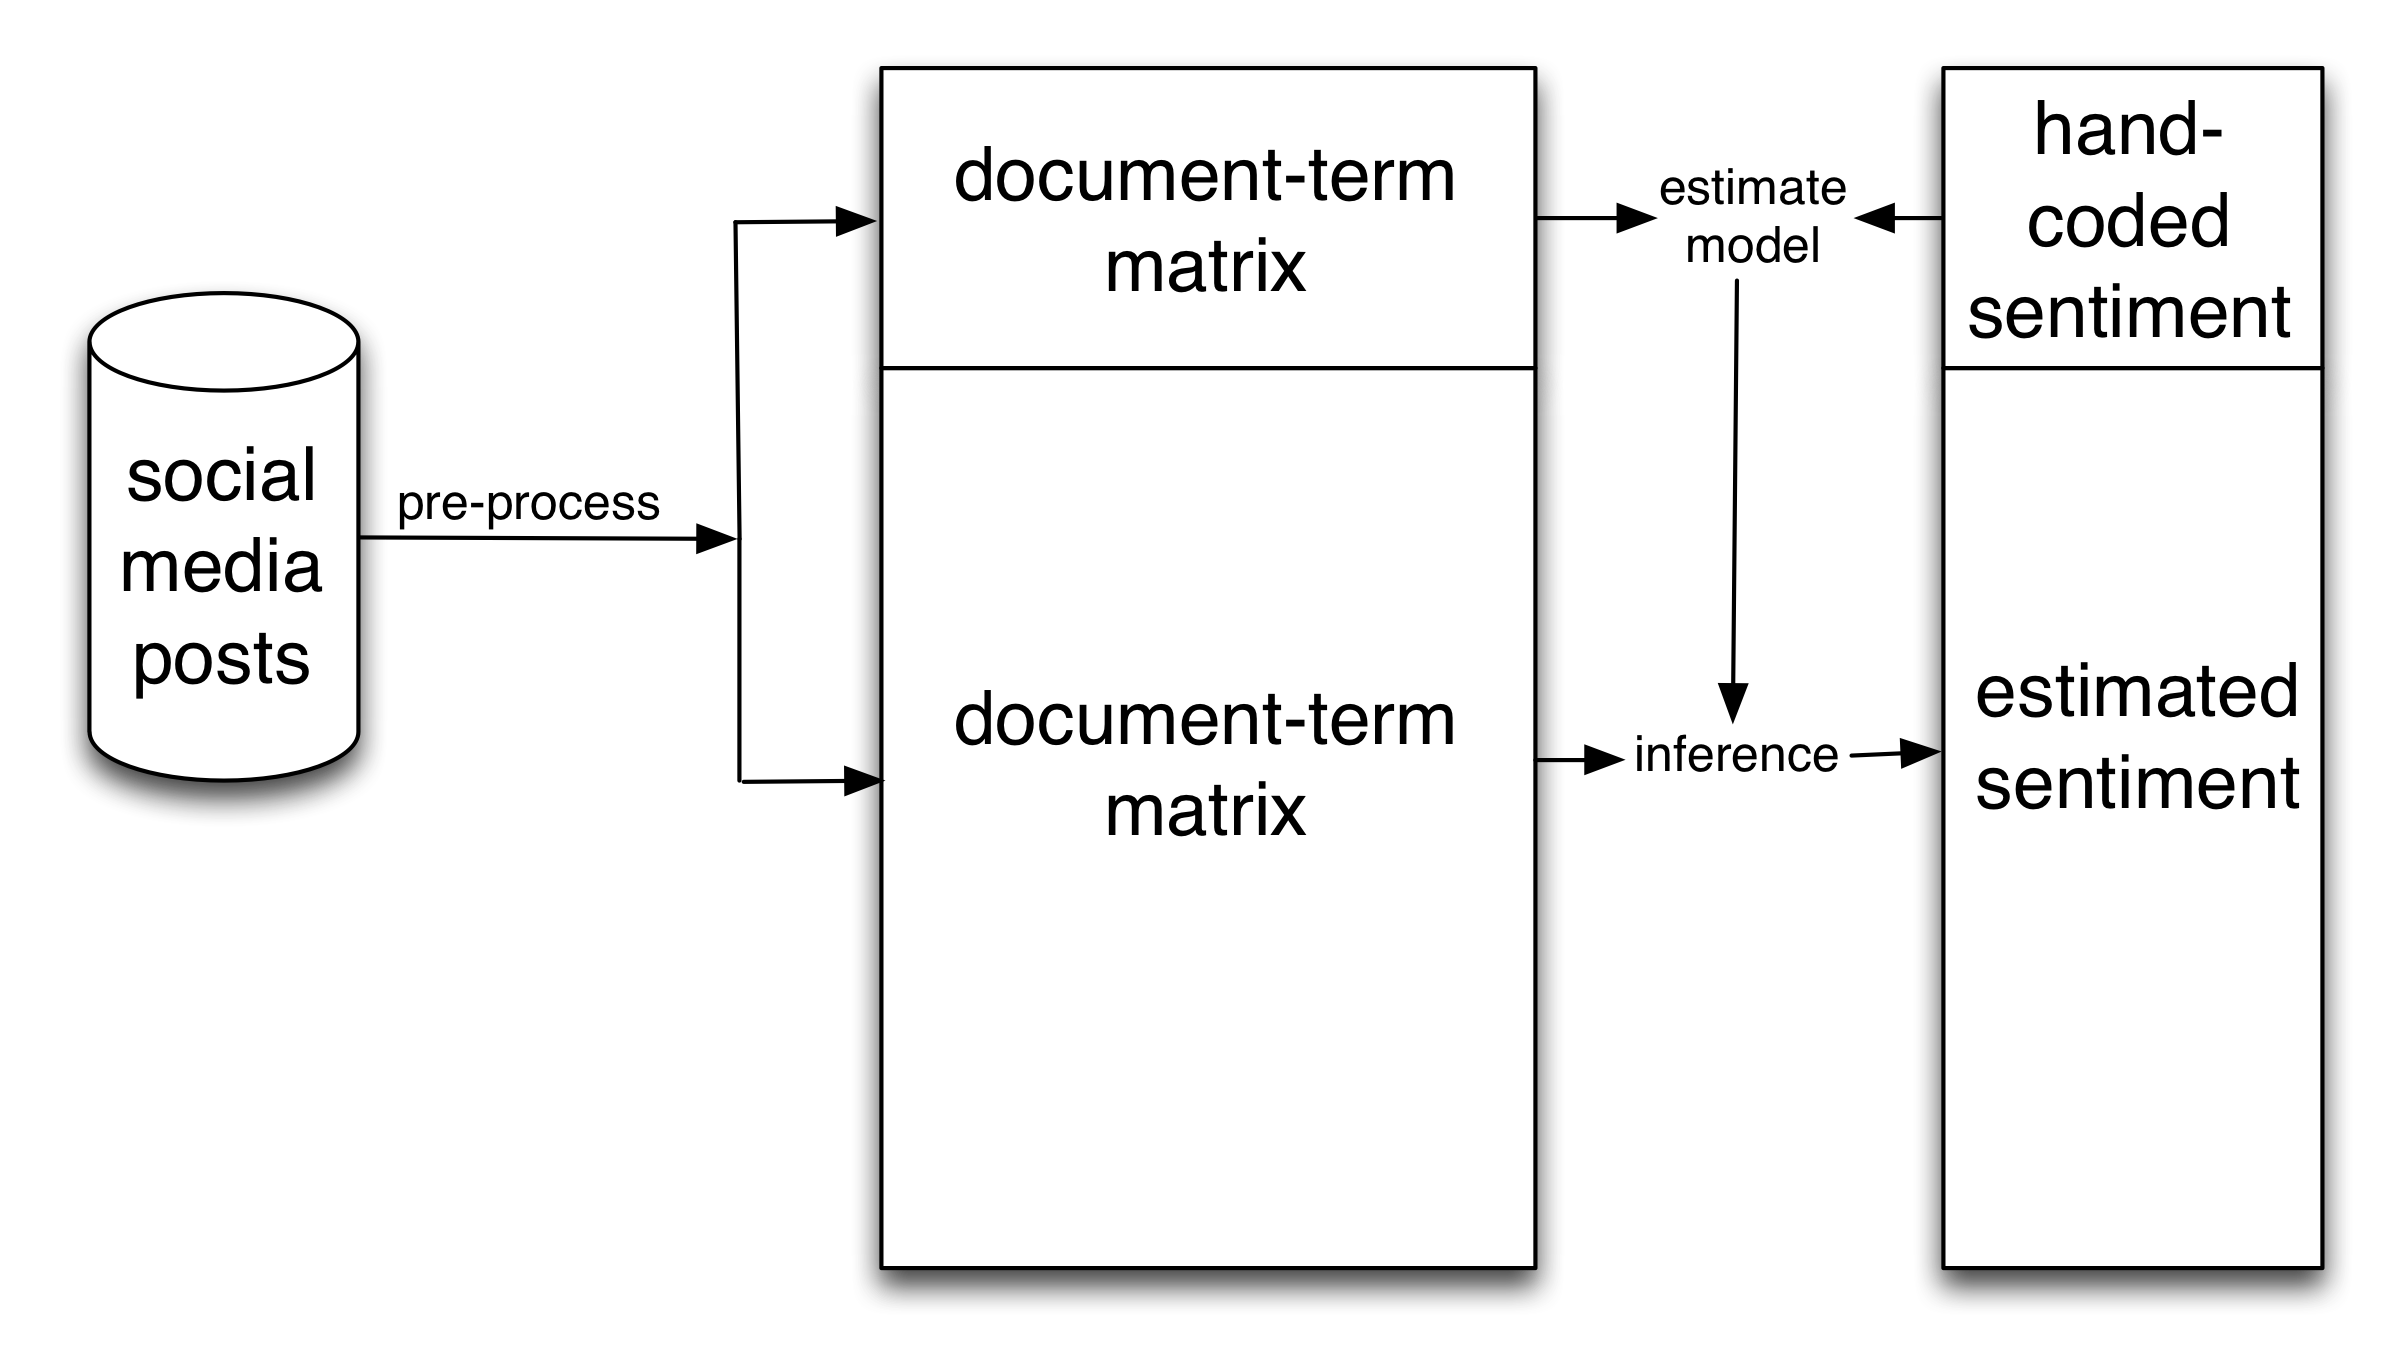
\includegraphics[width=0.9\textwidth]{figures/king_how_2013_schematic}
\end{center}
\vf
See Chapter 2 of Salganik (2016)
\end{frame}
%%%%%%%%%%%%%%%%%%%%%%%%%%%
\begin{frame}

\begin{center}
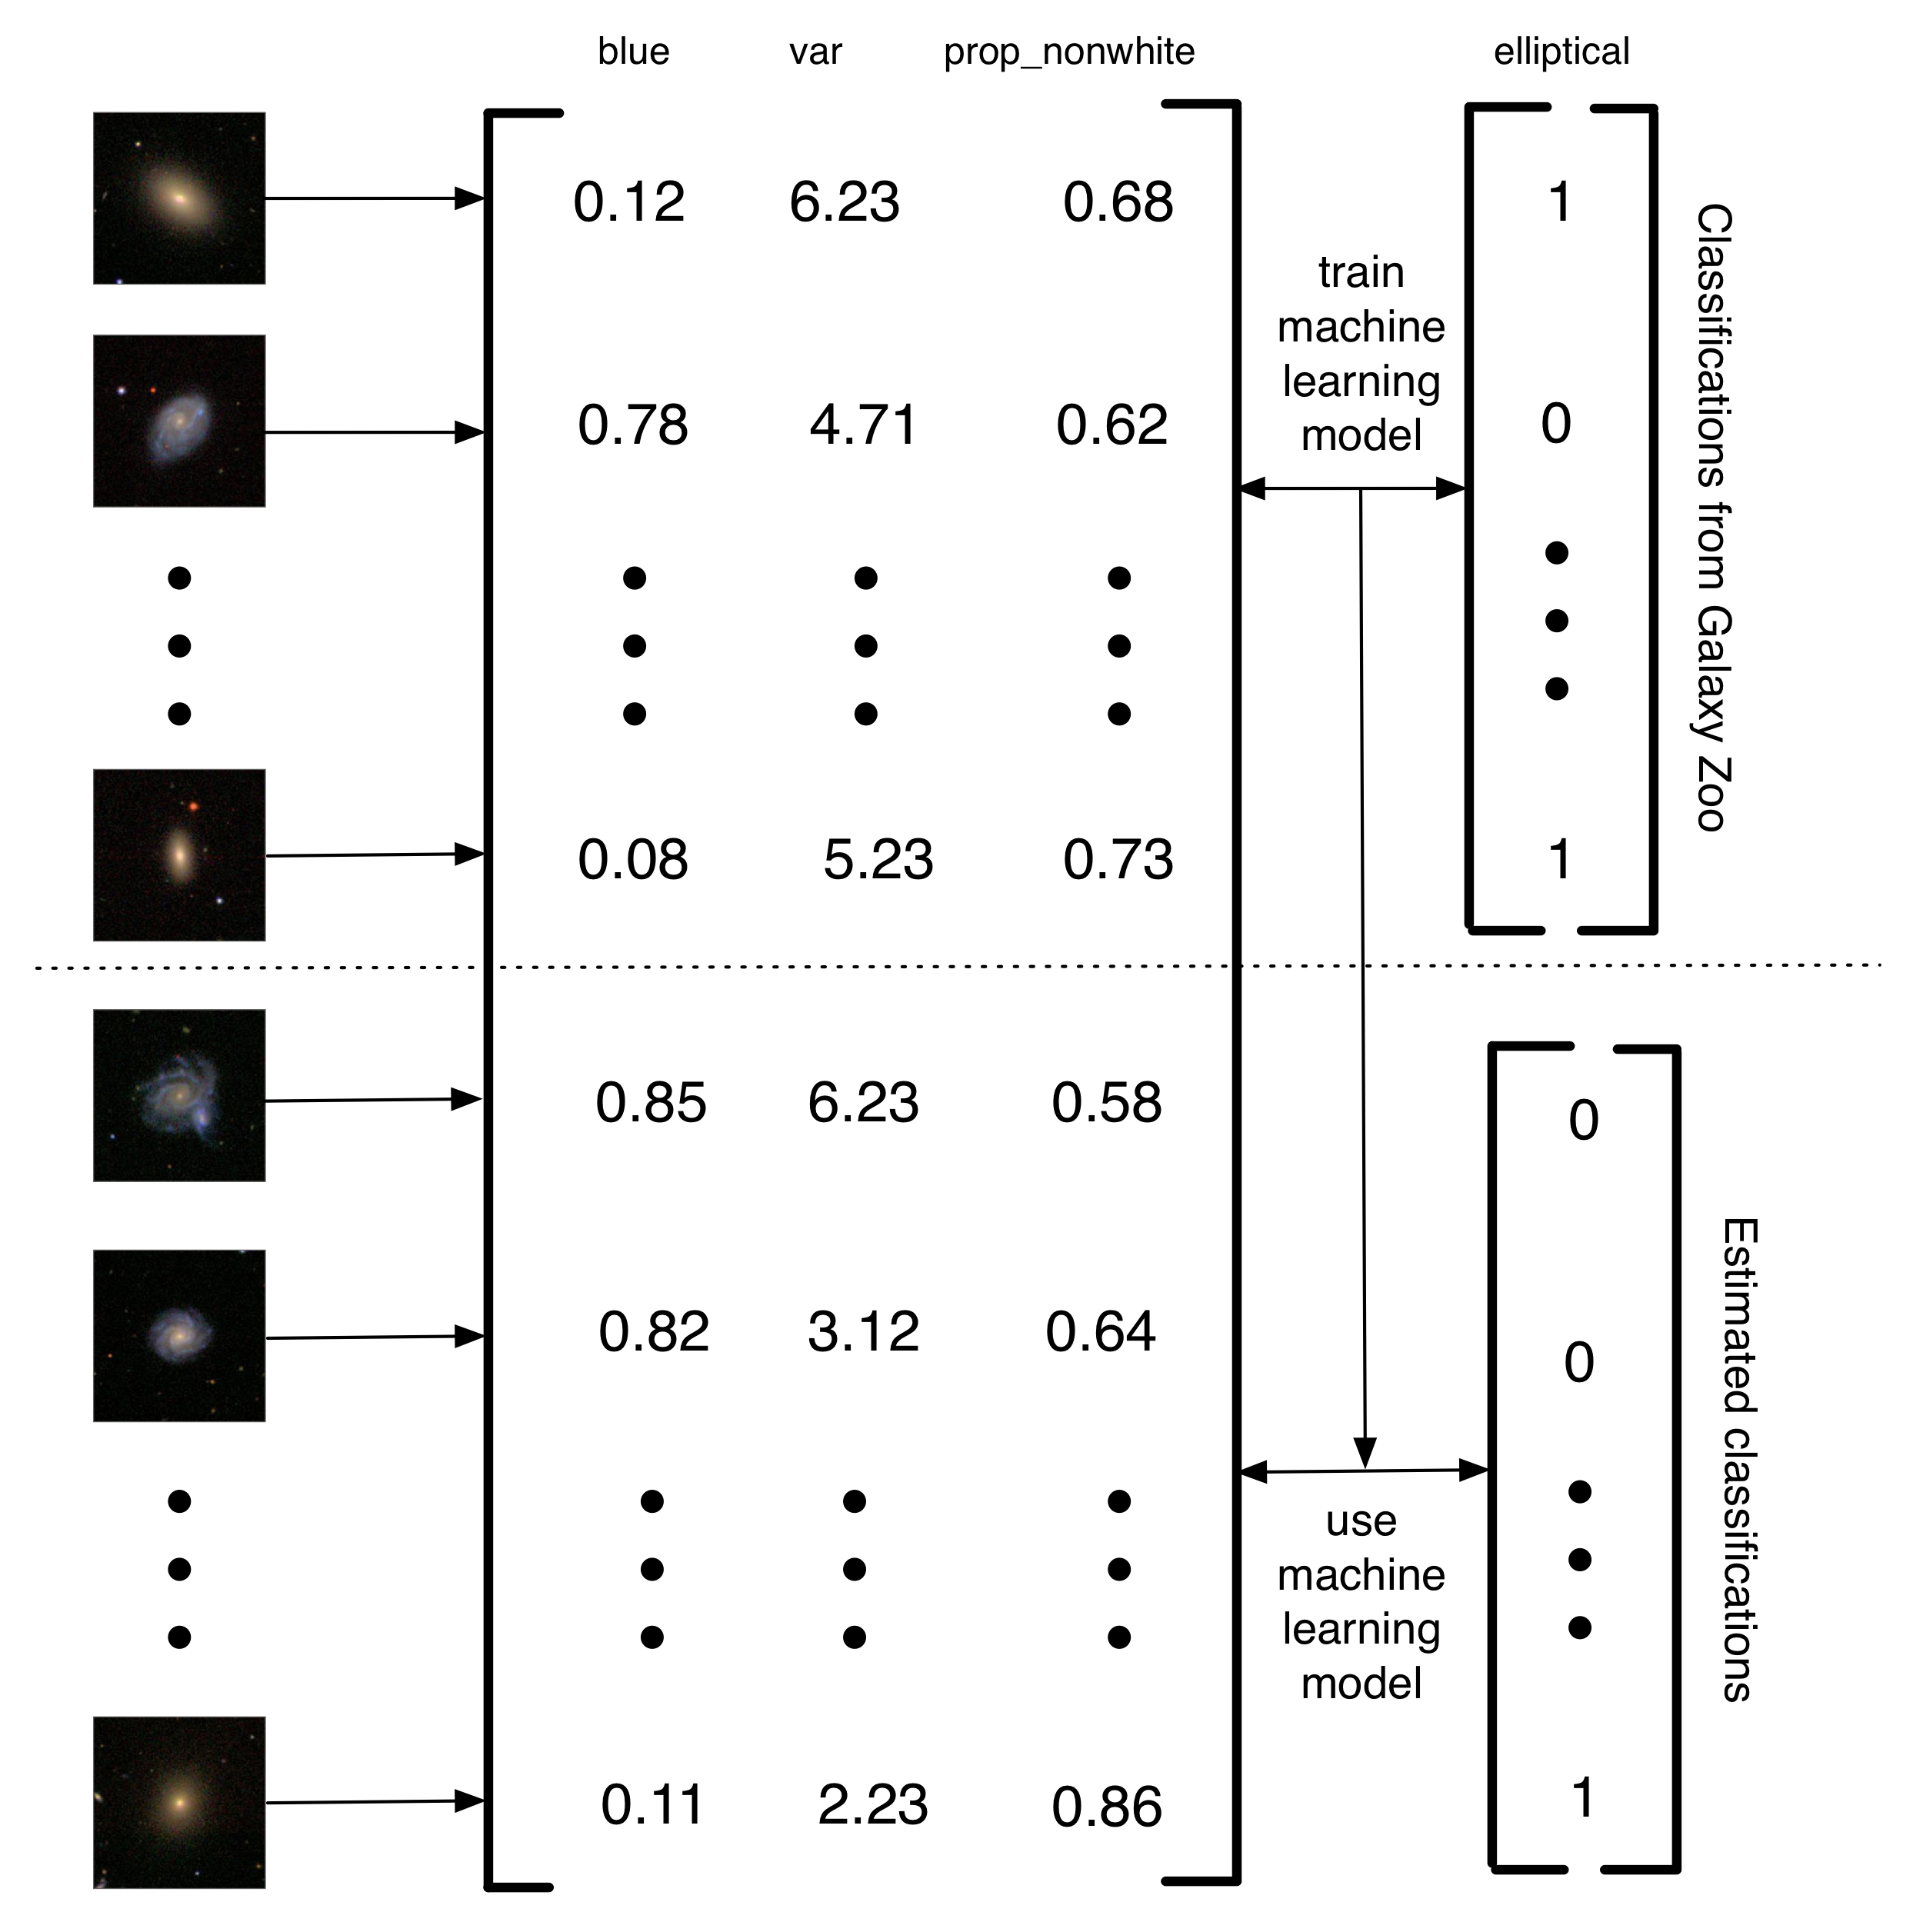
\includegraphics[height=0.9\textheight]{figures/gz_banerji_schematic}
\end{center}
\vf
See Chapter 5 of Salganik (2016)
\end{frame}
%%%%%%%%%%%%%%%%%%%%%%%%%%%
\begin{frame}

Supervised learning:\\
Lots of input-output pairs; goal is to develop a function that will predict the output from the input

\end{frame}
%%%%%%%%%%%%%%%%%%%%%%%%
\begin{frame}

\Large{
\begin{center}
What if rather than engineering the features you could ``learn'' them automatically?
\end{center}
}
\end{frame}
%%%%%%%%%%%%%%%%%%%%%%%%
\begin{frame}

\begin{center}
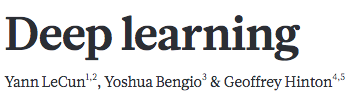
\includegraphics[width=0.8\textwidth]{figures/lecunn_deep_2015}
\end{center}
\vf
\url{http://dx.doi.org/10.1038/nature14539}
\end{frame}
%%%%%%%%%%%%%%%%%%%%%%%%%%%
\begin{frame}

{\Large
\begin{center}
``Have you tried deep learning?''
\end{center}
}

\end{frame}
%%%%%%%%%%%%%%%%%%%%%%%%
\begin{frame}

Deep learning + poverty + space

\begin{center}
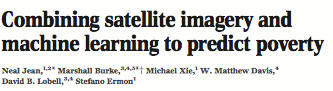
\includegraphics[width=0.9\textwidth]{figures/jean_combining_2016_title}
\end{center}

\end{frame}
%%%%%%%%%%%%%%%%%%%%%%%%%%%
\begin{frame}

Live demo:
\url{https://www.google.com/maps/place/Kigali,+Rwanda/@-1.9546259,30.0345059,26517m/data=!3m2!1e3!4b1!4m5!3m4!1s0x19dca4258ed8e797:0xf32b36a5411d0bc8!8m2!3d-1.9705786!4d30.1044288}

\end{frame}
%%%%%%%%%%%%%%%%%%%%%%%%%%%
\begin{frame}

But, most people had been using night lights
\begin{center}
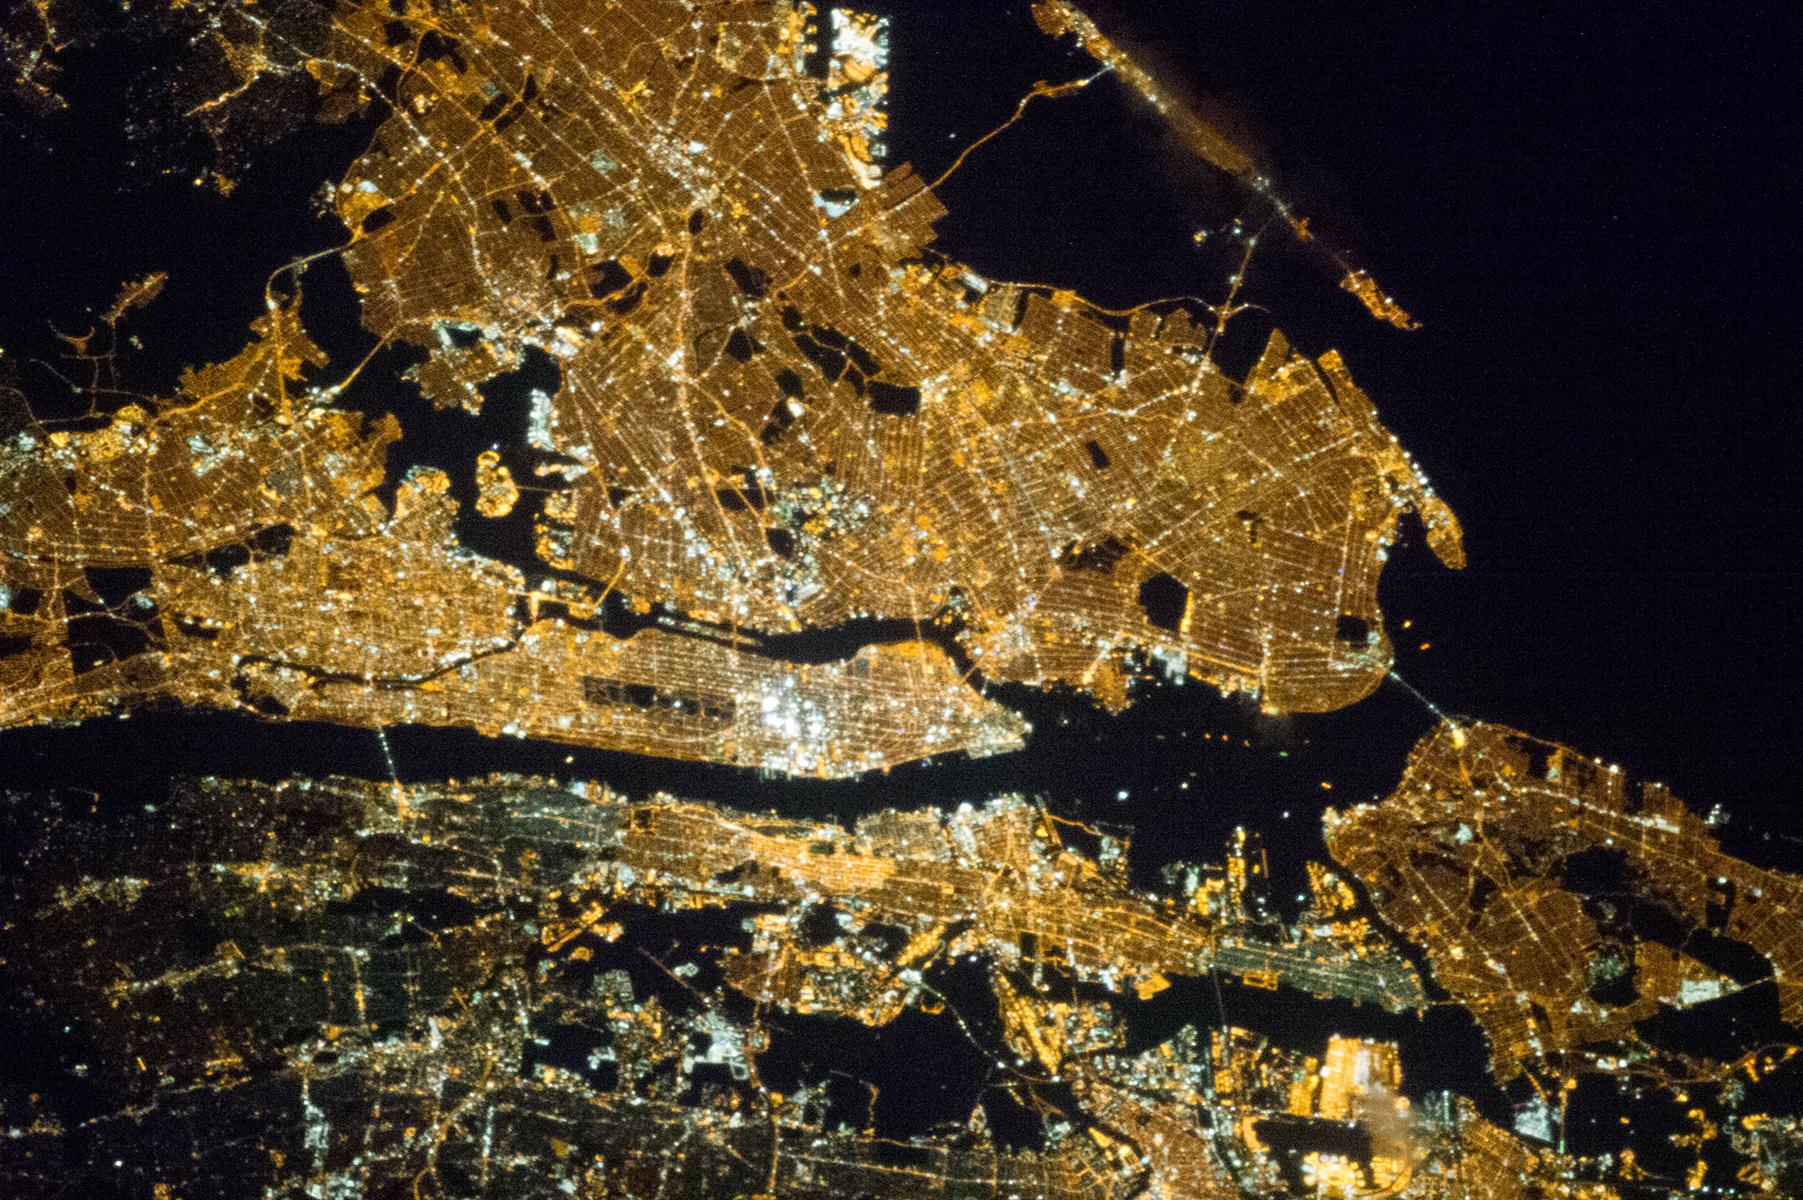
\includegraphics[width=0.7\textwidth]{figures/nyc_night}
\end{center}

\vf
\url{https://www.nasa.gov/multimedia/imagegallery/image_feature_2480.html}
\end{frame}
%%%%%%%%%%%%%%%%%%%%%%%%%%%
\begin{frame}

Nightlights + survey data to estimate wealth in places without surveys

\end{frame}
%%%%%%%%%%%%%%%%%%%%%%%%%%%
\begin{frame}

Jean et al. (2016):\\
Day pictures + Nightlights + survey data to estimate wealth in places without surveys

\end{frame}
%%%%%%%%%%%%%%%%%%%%%%%%%%%
\begin{frame}

\begin{center}
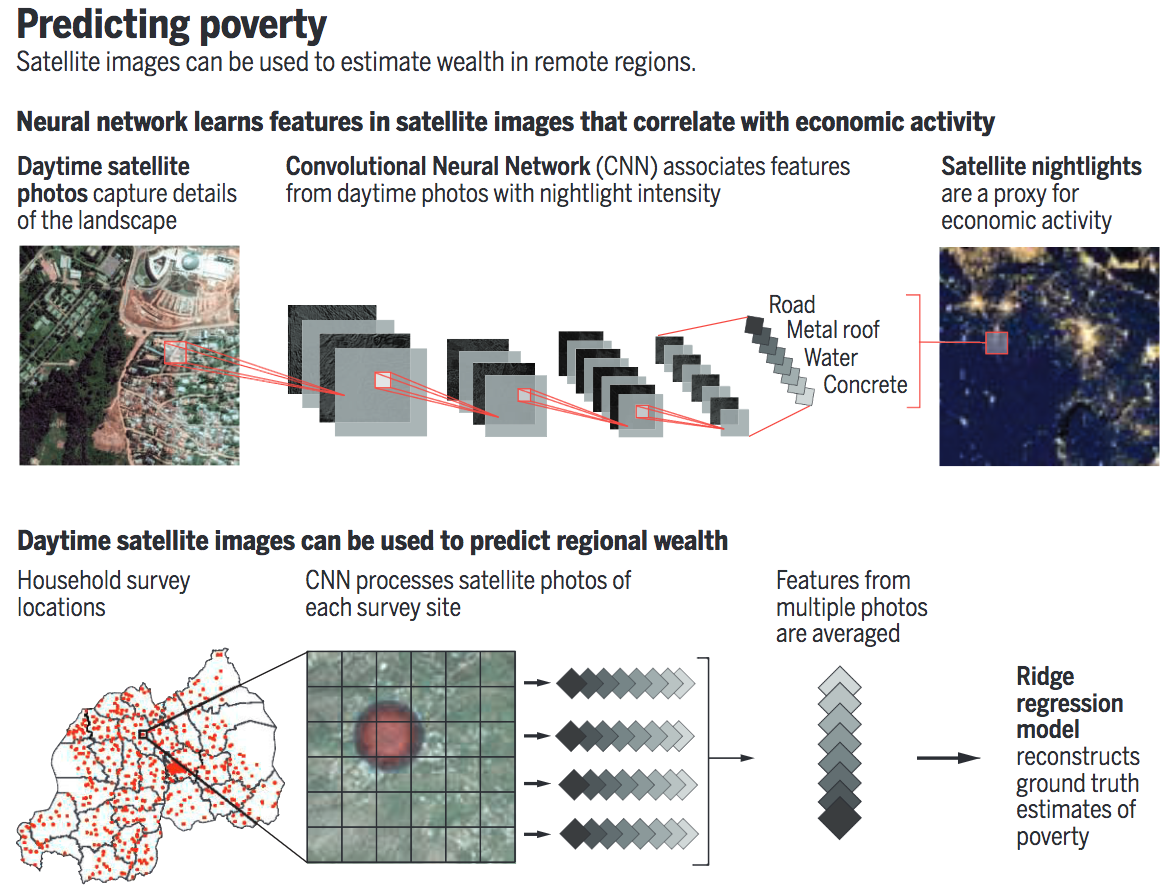
\includegraphics[width=0.4\textwidth]{figures/blumenstock_fighting_2016_fig}
\end{center}

\begin{itemize}
\item Start with CNN pretrained on ImageNet (e.g. hampsters and weasels)
\pause
\item Train CNN to predict nightlights from day pictures (lots of training data)
\end{itemize}

\end{frame}
%%%%%%%%%%%%%%%%%%%%%%%%%%%
\begin{frame}

\begin{center}
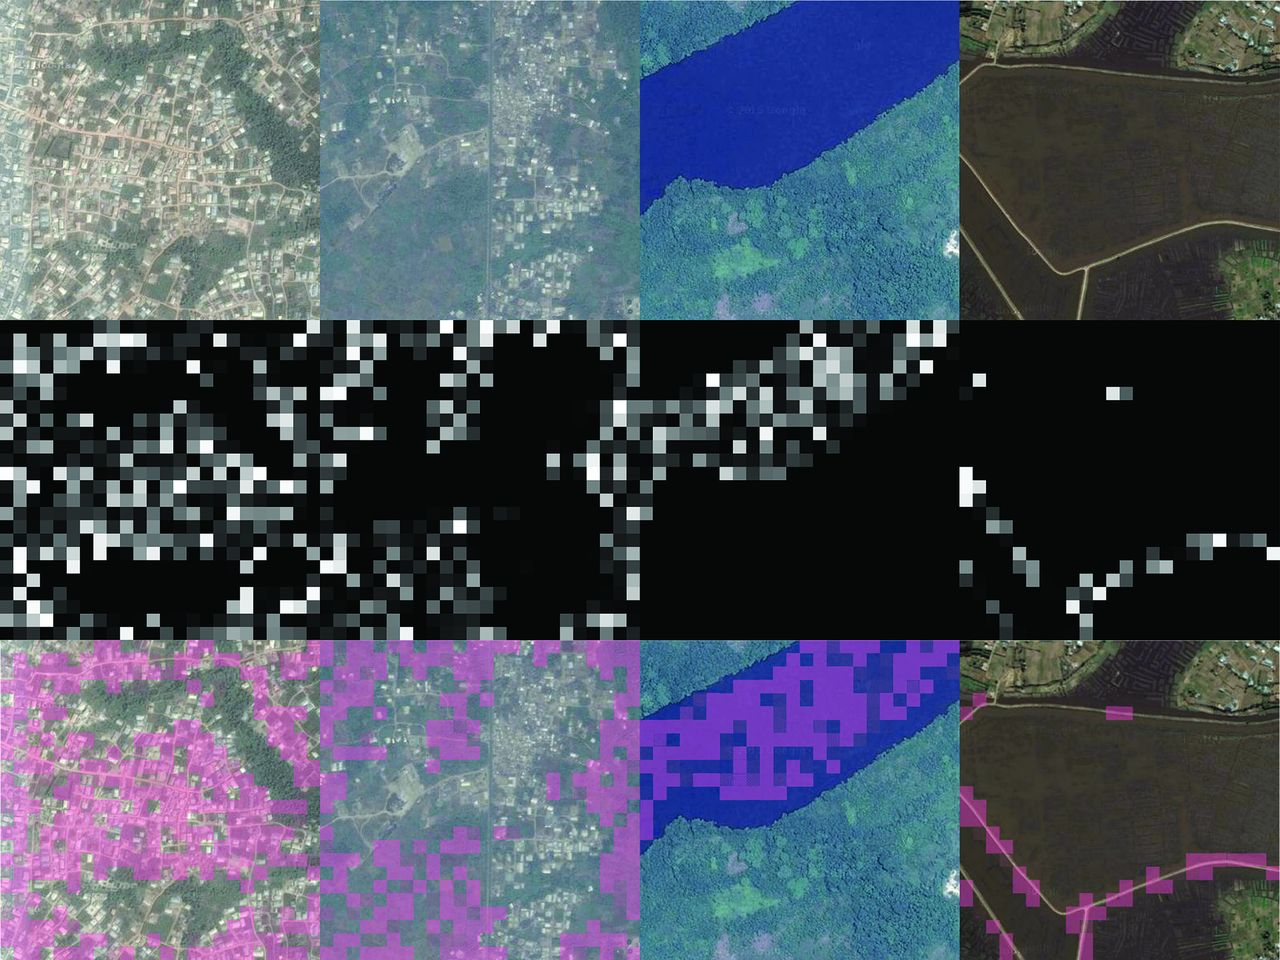
\includegraphics[width=0.7\textwidth]{figures/jean_combining_2016_fig2}
\end{center}

\end{frame}
%%%%%%%%%%%%%%%%%%%%%%%%%%%
\begin{frame}

\begin{center}
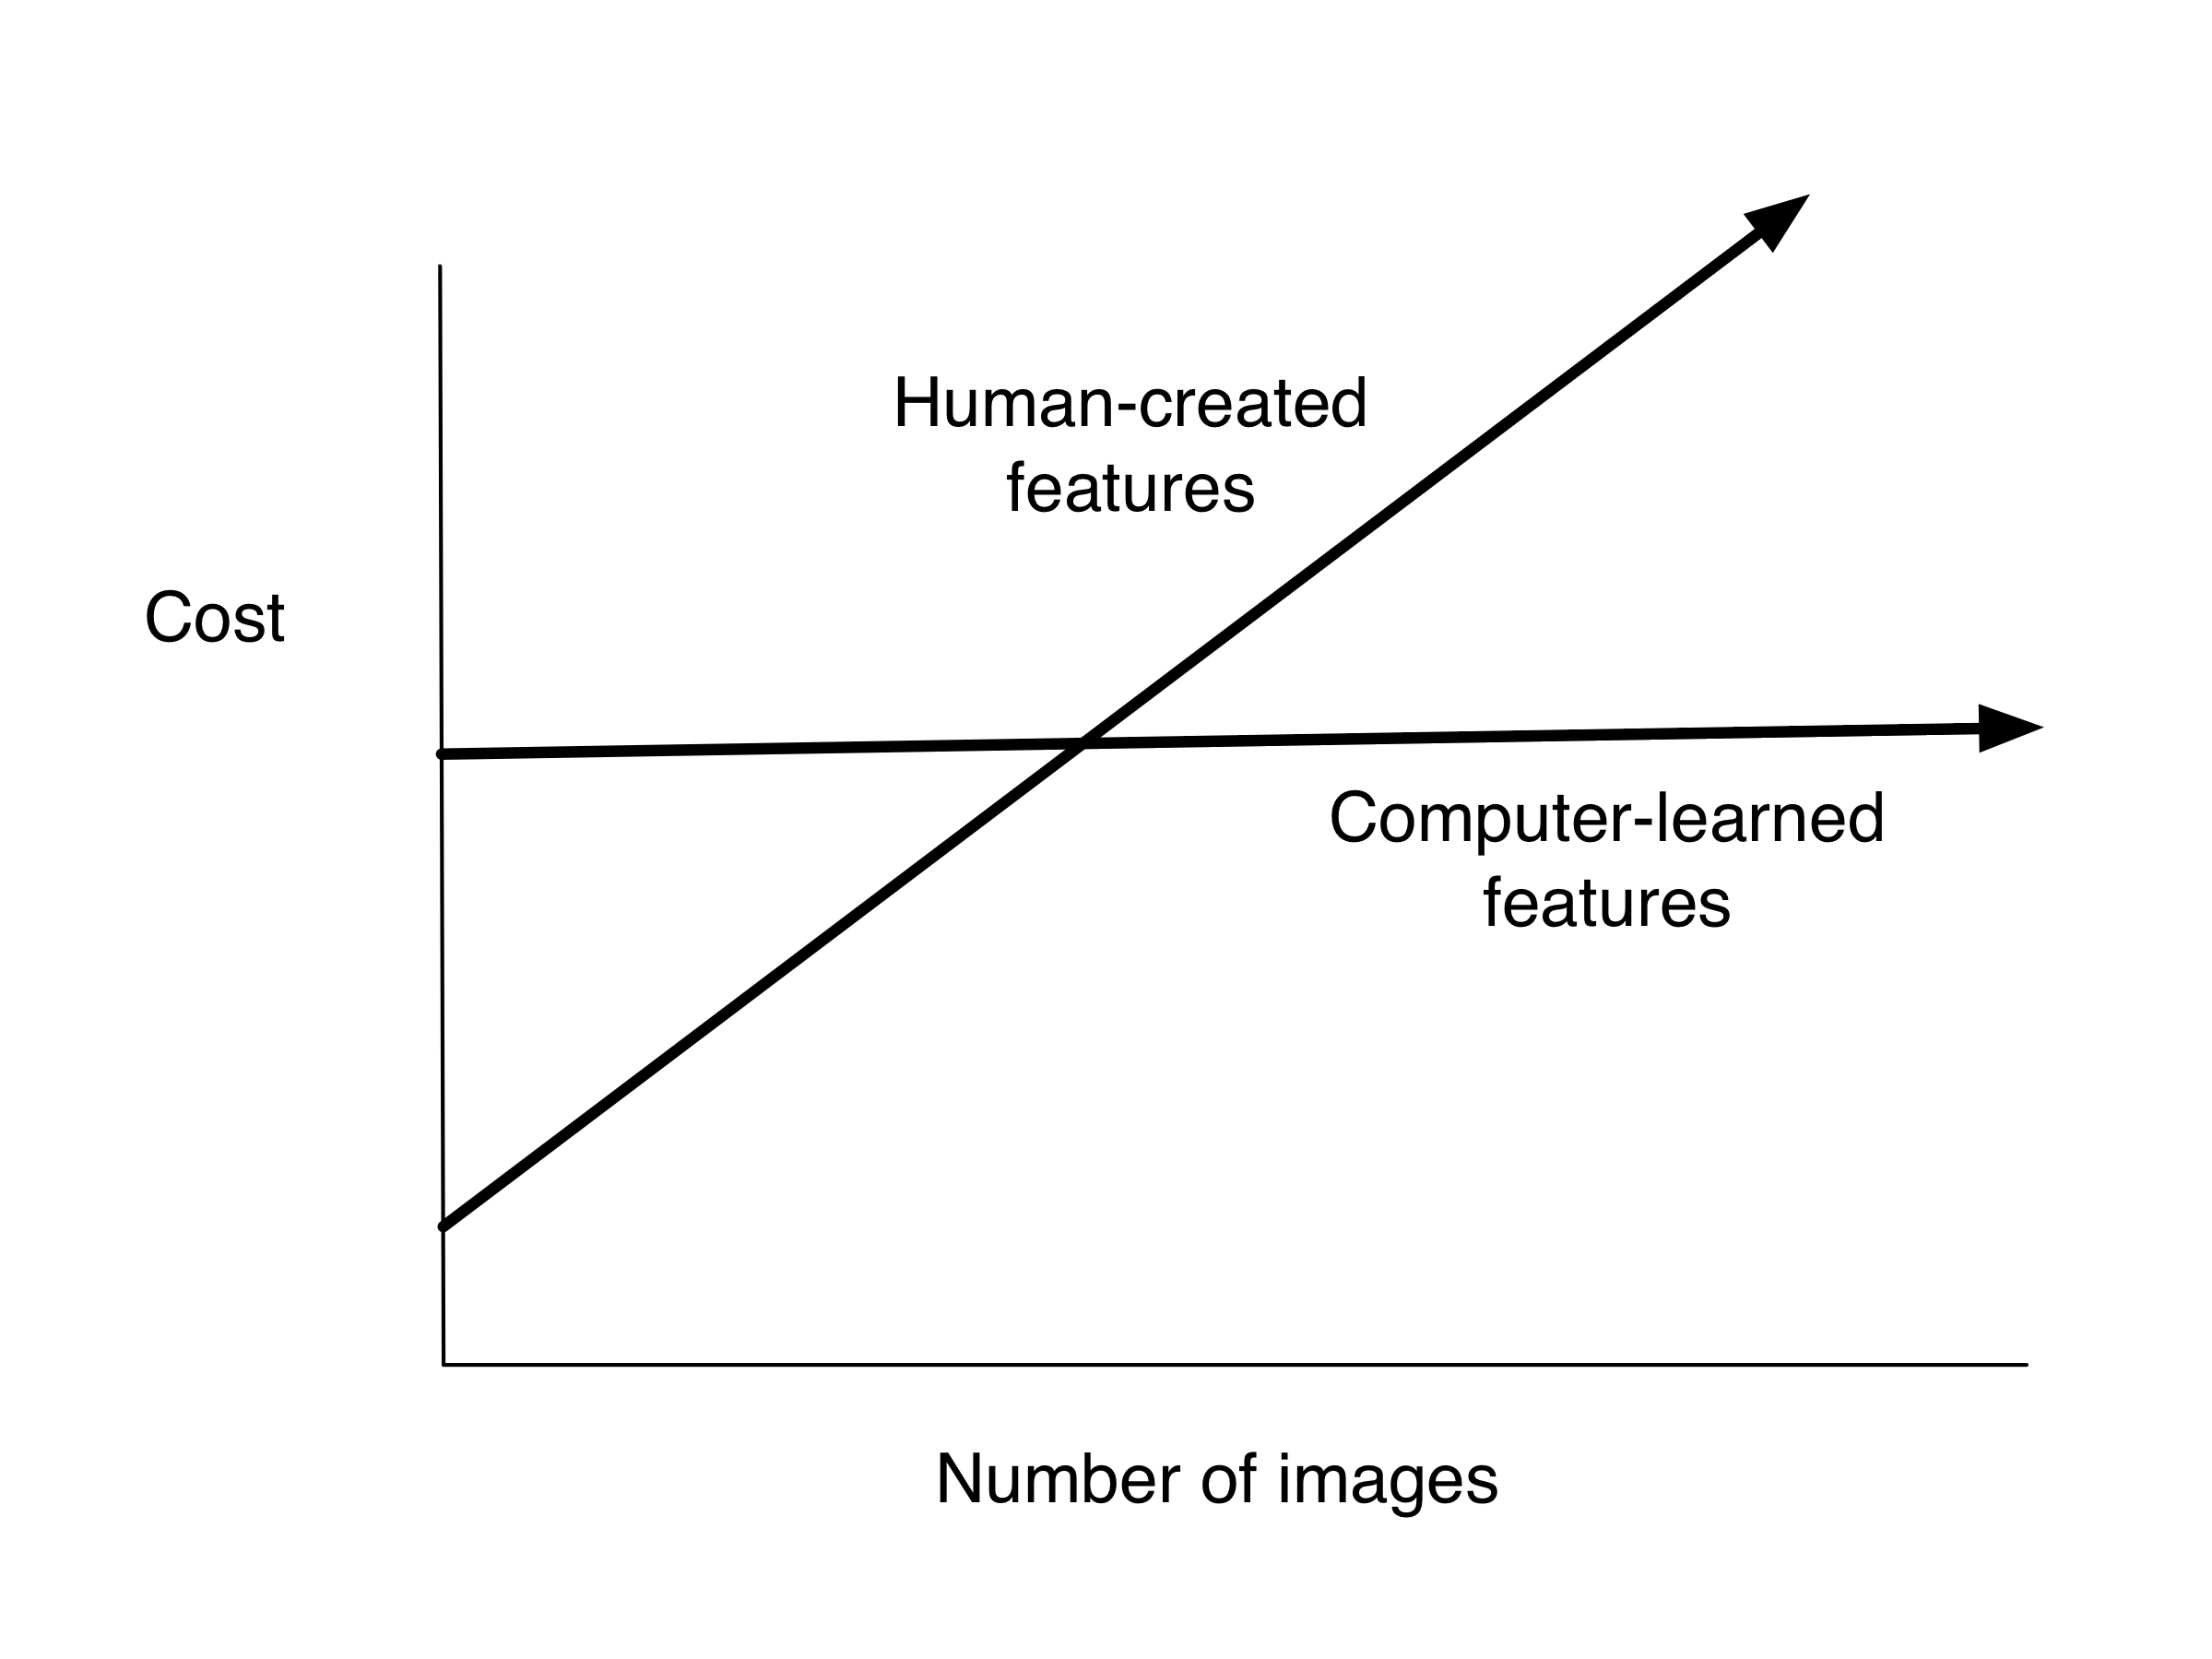
\includegraphics[width=0.7\textwidth]{figures/zero_variable_cost_features}
\end{center}

\end{frame}
%%%%%%%%%%%%%%%%%%%%%%%%%%%
\begin{frame}

\begin{itemize}
\item Start with CNN pretrained on ImageNet (e.g. hamsters and weasels)
\pause
\item Train CNN to predict nightlights from day pictures (lots of training data)
\pause
\item Take features from CNN and train ridge regression to predict cluster mean survey response
\end{itemize}

\end{frame}
%%%%%%%%%%%%%%%%%%%%%%%%%%%
\begin{frame}

\begin{center}
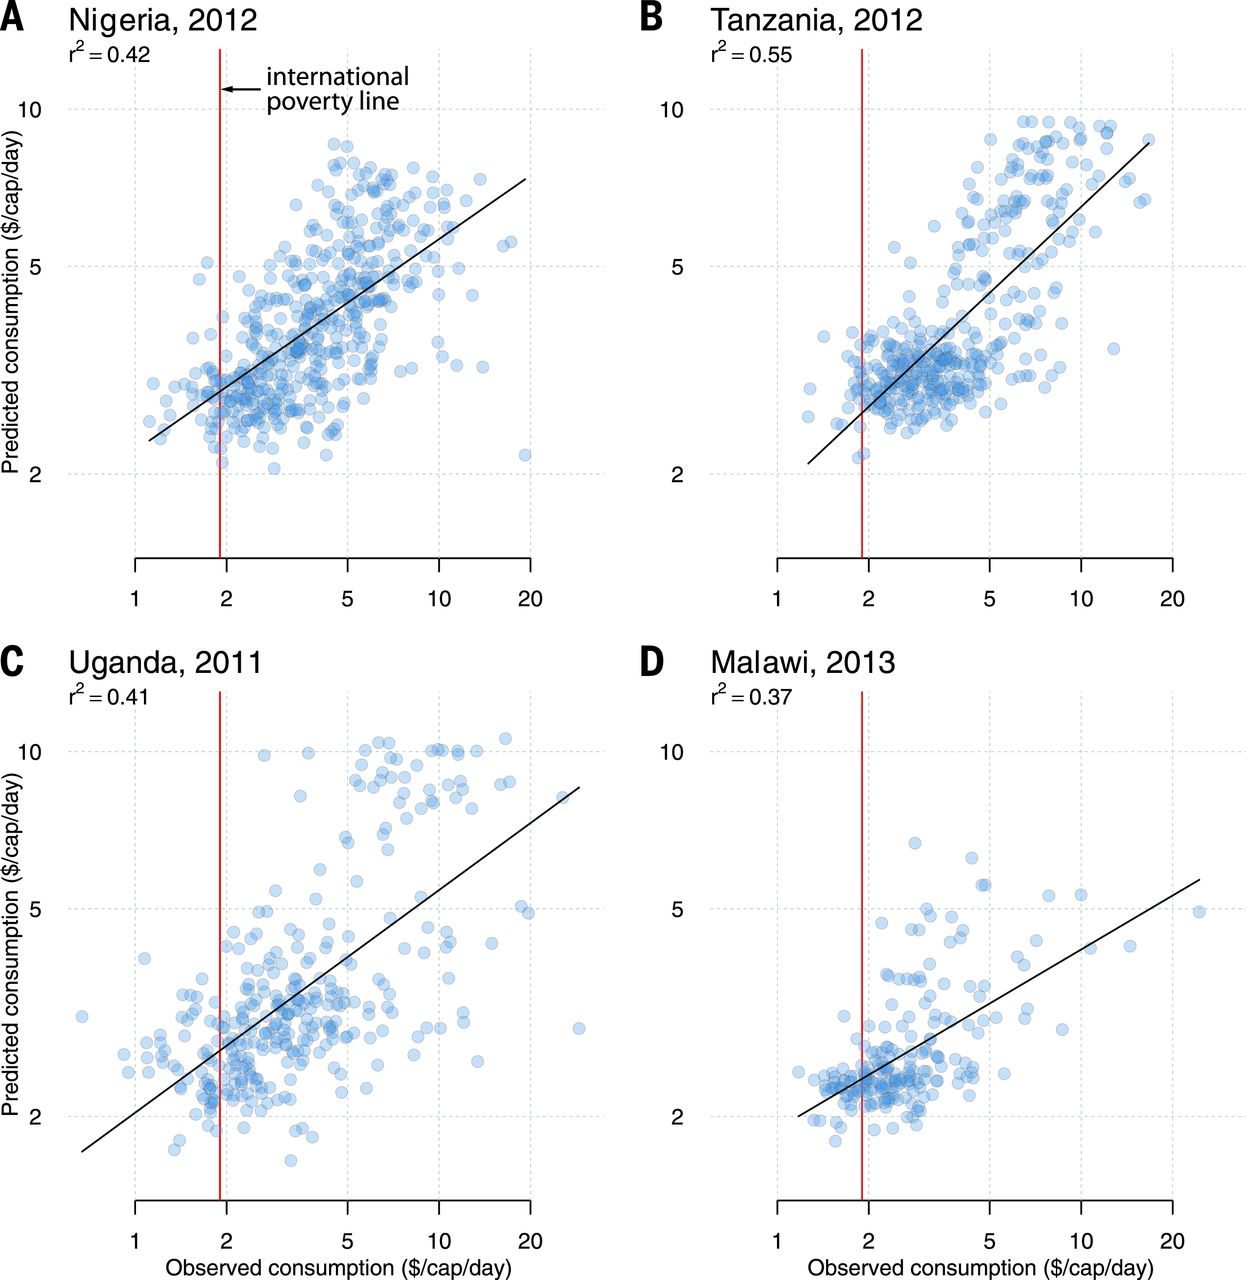
\includegraphics[width=0.5\textwidth]{figures/jean_combining_2016_fig3}
\end{center}
\vf
\textcolor{green}{How could this figure be improved?}

\end{frame}
%%%%%%%%%%%%%%%%%%%%%%%%%%%
\begin{frame}

\begin{center}
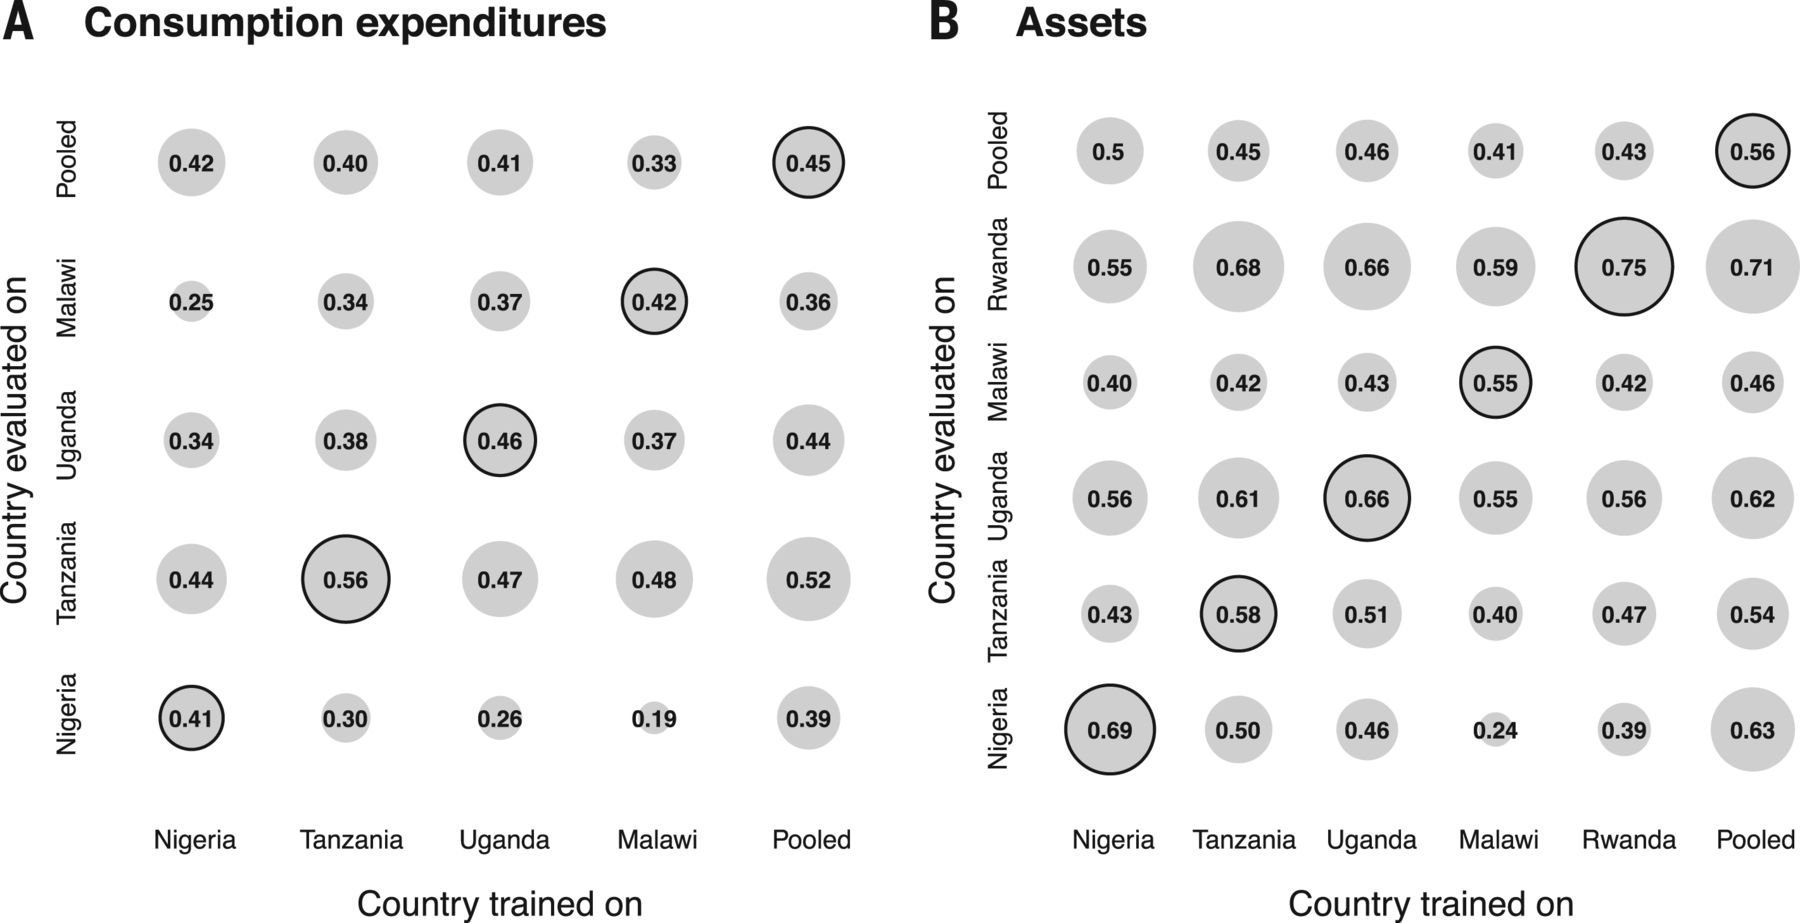
\includegraphics[width=0.9\textwidth]{figures/jean_combining_2016_fig5}
\end{center}

\end{frame}
%%%%%%%%%%%%%%%%%%%%%%%%%%%
\begin{frame}

\begin{columns}
\begin{column}{0.5\textwidth}
\begin{center}
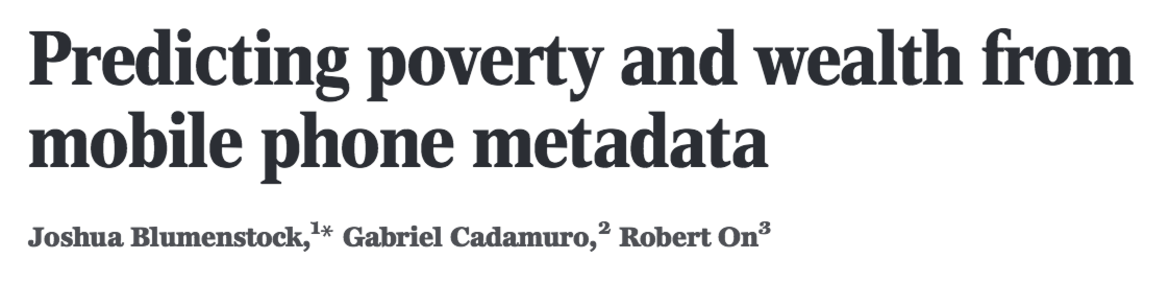
\includegraphics[width=0.9\textwidth]{figures/blumenstock_predicting_2015_title}\\
Readymade + Custommade
\end{center}
\end{column}
\begin{column}{0.5\textwidth}  
\begin{center}
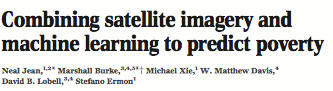
\includegraphics[width=0.9\textwidth]{figures/jean_combining_2016_title}\\
Readymade + Readymade + (Quasi) Custommade
\end{center}
\end{column}
\end{columns}

\end{frame}
%%%%%%%%%%%%%%%%%%%%%%%%%%%
\begin{frame}

\textcolor{green}{Both Blumenstock et al (2015) and Jean et al (2016) estimate poverty in Africa?  Compare the strengths and weaknesses of the approaches.}

\end{frame}
%%%%%%%%%%%%%%%%%%%%%%%%%%%
\begin{frame}

\begin{columns}

\begin{column}{0.5\textwidth}  
\begin{center}
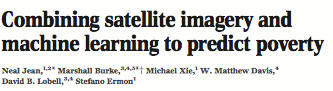
\includegraphics[width=0.9\textwidth]{figures/jean_combining_2016_title}\\
Uses Readymade linked to Researcher-Custommade
\end{center}
\end{column}
\begin{column}{0.5\textwidth}
\begin{center}
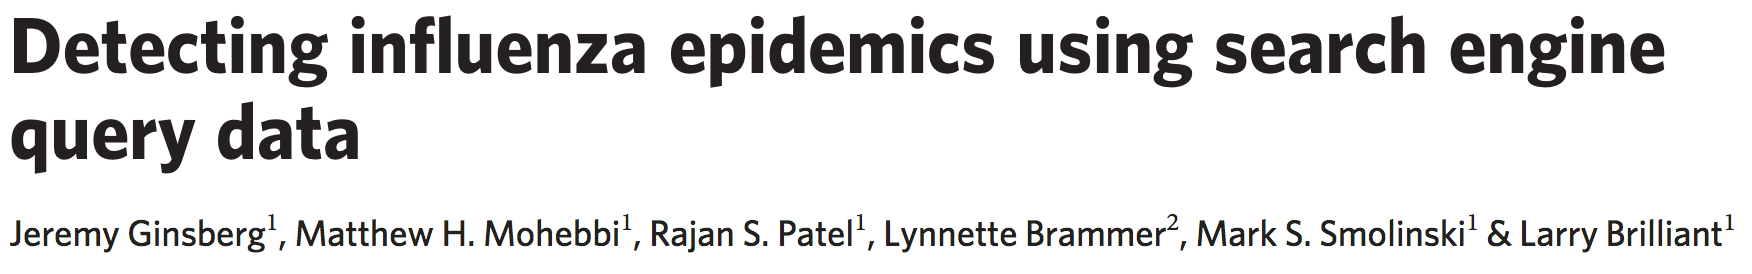
\includegraphics[width=0.9\textwidth]{figures/ginsberg_detecting_2009_title}\\
Uses Readymade linked to Researcher-Custommade
\end{center}
\end{column}
\end{columns}

\end{frame}
%%%%%%%%%%%%%%%%%%%%%%%%%%%
\begin{frame}

\textcolor{green}{Is there a role for individual researchers collecting data in the age of the Readymades and Quasi Custommades?}

\end{frame}
%%%%%%%%%%%%%%%%%%%%%%%%%%%
\begin{frame}

\textcolor{green}{How should governments collect large general purpose dataset if they will be combined with Readymades?}

\end{frame}
%%%%%%%%%%%%%%%%%%%%%%%%%%%

\end{document}
